\documentclass[a4paper,11pt]{article}

\usepackage[
    left=1.5cm,
    right=1.5cm,
    top=0cm,
    bottom=1.8cm,
    footskip=1.1cm
]{geometry}

\usepackage{montserrat}
\renewcommand{\familydefault}{\sfdefault}
\usepackage[T1]{fontenc}
\usepackage{graphicx}
\usepackage{xcolor}
\usepackage{tikz}
\usetikzlibrary{calc,positioning,shapes.geometric,shadows}
\usepackage[most]{tcolorbox}
\usepackage{multicol}
\usepackage{enumitem}
\usepackage{fancyhdr}
\usepackage{tabularx}
\usepackage{colortbl}
\usepackage{hyperref}
\usepackage{eso-pic}

% Declare graphics paths for seamless resolution
\graphicspath{{images/}{profile images/}{images/hero/}{images/aigenerated/}{images/projects/civilworks/}{images/projects/roadsandsurfacing/}{images/projects/earthworks/}{images/projects/buildingconstruction/}}

% =================================================
% BRAND PALETTE (MAKHASWA OFFICIAL: NAVY, BLUE, WHITE, BLACK)
% =================================================

\definecolor{mhnavy}{HTML}{082D5A}        % Primary Brand Deep Navy
\definecolor{mhnavy2}{HTML}{0C3A6D}       % Mid Corporate Navy
\definecolor{mhnavy3}{HTML}{124884}       % Accent Navy
\definecolor{mhblue}{HTML}{1A56A0}        % Crisp Corporate Blue
\definecolor{mhbluebright}{HTML}{0066CC}  % Bright Blue Accent
\definecolor{mhbluelight}{HTML}{F0F4FA}   % Soft Light Blue Background
\definecolor{mhgold}{HTML}{C8A951}        % Subtle Gold Keyline

\definecolor{mhoffwhite}{HTML}{F8FAFC}    % Clean Slate Off-White
\definecolor{mhlightgray}{HTML}{E2E8F0}   % Clean Minimal Border
\definecolor{mhtext}{HTML}{1E293B}        % Charcoal Dark Body Text
\definecolor{mhtextmuted}{HTML}{64748B}   % Slate Gray Subtitle Text

\pagecolor{white}
\color{mhtext}

% =================================================
% HYPERLINK SETTINGS
% =================================================

\hypersetup{
    colorlinks=true,
    linkcolor=mhnavy,
    urlcolor=mhnavy,
    citecolor=mhblue
}

% =================================================
% REUSABLE TCOLORBOX STYLES & COMPONENTS
% =================================================

% Clean Brand Card for General Sections
\newtcolorbox{brandcard}[2][]{
    enhanced,
    colback=white,
    colframe=mhlightgray,
    boxrule=0.8pt,
    arc=4pt,
    title={\bfseries\color{mhnavy} #2},
    colbacktitle=mhoffwhite,
    coltitle=mhnavy,
    fonttitle=\bfseries\normalsize,
    attach boxed title to top left={yshift=-2.5mm, xshift=4mm},
    boxed title style={boxrule=0.8pt, colframe=mhnavy, arc=2pt, colback=mhoffwhite},
    left=10pt,
    right=10pt,
    top=12pt,
    bottom=10pt,
    drop shadow=black!3,
    #1
}

% Stat Badge for Key Numbers & Highlights
\newtcolorbox{statbadge}[1][]{
    enhanced,
    colback=mhoffwhite,
    colframe=mhlightgray,
    boxrule=0.8pt,
    arc=4pt,
    halign=center,
    valign=center,
    left=4pt,
    right=4pt,
    top=8pt,
    bottom=8pt,
    height=2.5cm,
    borderline south={2.5pt}{0pt}{mhnavy},
    drop shadow=black!3,
    #1
}

% Solid Logo Badge on Dark Backgrounds
\newtcolorbox{logobadge}[1][]{
    enhanced,
    colback=white,
    colframe=mhnavy2,
    boxrule=1pt,
    arc=4pt,
    boxsep=3pt,
    left=8pt,
    right=8pt,
    top=6pt,
    bottom=6pt,
    halign=center,
    valign=center,
    drop shadow=black!20,
    #1
}

% Dark Service Box for Engineering Disciplines
\newtcolorbox{darkservice}[1][]{
    enhanced,
    colback=mhnavy,
    colframe=mhnavy,
    boxrule=0pt,
    arc=4pt,
    coltext=white,
    left=10pt,
    right=10pt,
    top=10pt,
    bottom=10pt,
    borderline west={3pt}{0pt}{mhblue},
    drop shadow=black!6,
    #1
}

% Highlight Feature Card
\newtcolorbox{featurecard}[2][]{
    enhanced,
    colback=mhoffwhite,
    colframe=mhlightgray,
    boxrule=0.8pt,
    arc=4pt,
    title={\bfseries\color{mhnavy} #2},
    colbacktitle=mhoffwhite,
    coltitle=mhnavy,
    fonttitle=\bfseries\small,
    attach boxed title to top left={yshift=-2mm, xshift=3mm},
    boxed title style={boxrule=0.6pt, colframe=mhblue, arc=2pt},
    left=8pt,
    right=8pt,
    top=10pt,
    bottom=8pt,
    borderline west={2.5pt}{0pt}{mhnavy},
    #1
}

% Top Header Section Banner (Clean Navy with Crisp White & Blue Accent)
\newcommand{\sectionbanner}[2]{
    \begin{tikzpicture}[remember picture, overlay]
        \node[anchor=north west, inner sep=0pt] at (current page.north west) {
            \begin{tikzpicture}
                % Top Solid Navy Header
                \fill[mhnavy] (0,0) rectangle (\paperwidth, 3.5cm);
                % Subtle Clean Blue Line (No Rainbow / No Green / No Flags)
                \fill[mhblue] (0,0) rectangle (\paperwidth, 0.15cm);
            \end{tikzpicture}
        };
        % Right Solid Logo Accent in Header
        \node[anchor=north east] at ([xshift=-1.5cm, yshift=-0.55cm]current page.north east) {
            \begin{tcolorbox}[
                enhanced,
                colback=white,
                colframe=mhlightgray,
                boxrule=0.8pt,
                arc=3pt,
                boxsep=2pt,
                left=4pt, right=4pt, top=3pt, bottom=3pt,
                width=3.2cm,
                halign=center
            ]
                
\includegraphics[height=1.0cm, keepaspectratio]{images/logo.jpeg}
            \end{tcolorbox}
        };
    \end{tikzpicture}
    \vspace*{0.55cm}
    \noindent
    \hspace{0.1cm}
    \begin{minipage}{0.68\textwidth}
        {\fontsize{22pt}{26pt}\selectfont\bfseries\color{white} #1}\\[0.12cm]
        {\footnotesize\bfseries\color{mhbluelight} \MakeUppercase{#2}}
    \end{minipage}
    \vspace{1.05cm}
}

% =================================================
% FOOTER CONFIGURATION
% =================================================

\pagestyle{fancy}
\fancyhf{}
\renewcommand{\headrulewidth}{0pt}

\fancyfoot[L]{
    \fontsize{8pt}{10pt}\selectfont
    \color{mhtextmuted}
    \textbf{Makhaswa Holdings (Pty) Ltd}
    \ $\bullet$ \
    CIDB Grade 8 CE PE \ $\bullet$ \ Reg: K2017/307900/07
}

\fancyfoot[R]{
    \fontsize{8pt}{10pt}\selectfont
    \color{mhnavy}
    \textbf{\thepage}
}

% =================================================
% DOCUMENT START
% =================================================

\begin{document}

% =================================================
% PAGE 1 — COVER (CLEAN ASYMMETRICAL SPLIT WITH SOLID LOGO)
% =================================================

\begin{titlepage}
\thispagestyle{empty}

\begin{tikzpicture}[remember picture, overlay]

    % Base White Background
    \fill[white] (current page.north west) rectangle (current page.south east);

    % Right Imagery Panel (54% Width with Proportional Fit)
    \node[anchor=north east, inner sep=0pt] at (current page.north east) {
        \begin{tikzpicture}
            \clip (0,0) rectangle (0.54\paperwidth, \paperheight);
            \node[anchor=center, inner sep=0pt] at (0.27\paperwidth, 0.5\paperheight) {
                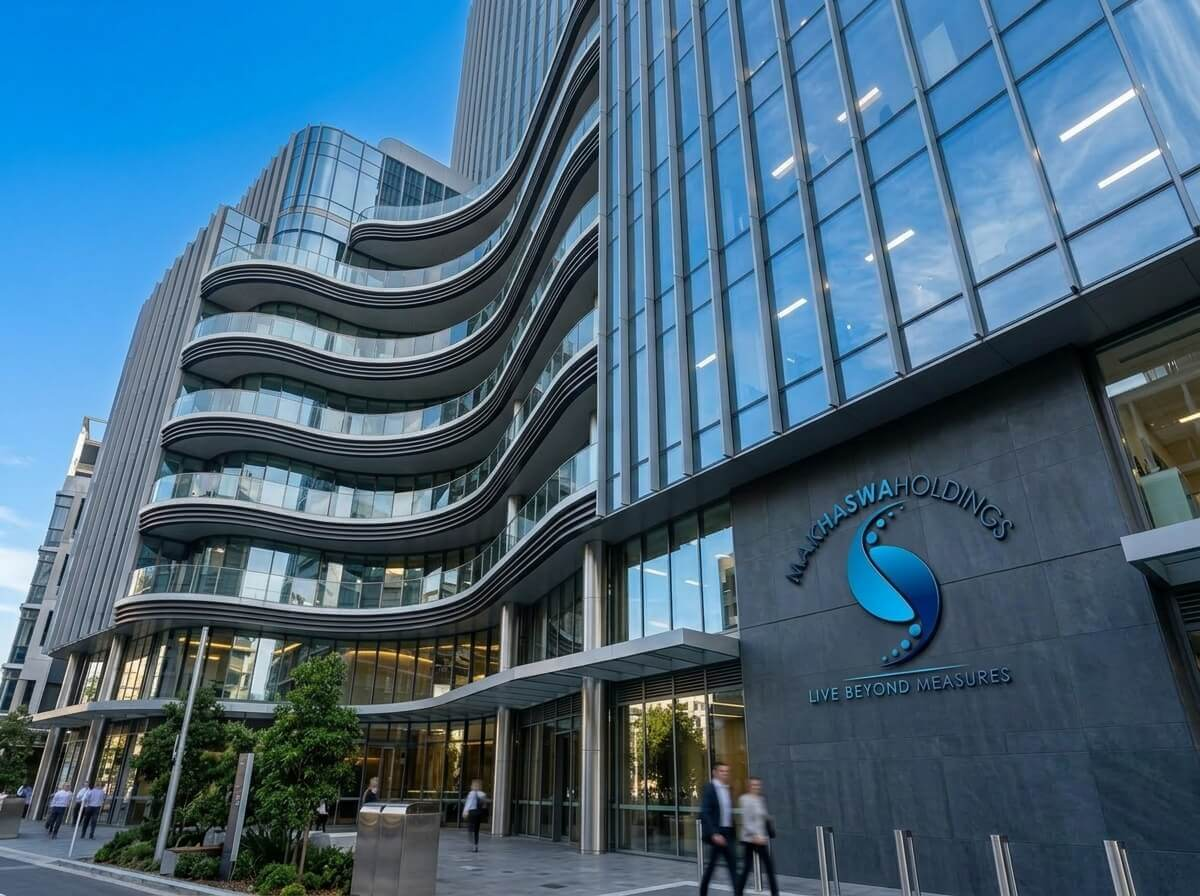
\includegraphics[
                    height=\paperheight,
                    keepaspectratio
                ]{images/makhaswa-building.jpeg}
            };
        \end{tikzpicture}
    };

    % Left Solid Deep Navy Panel (46% Width)
    \fill[mhnavy] (current page.north west) rectangle ([xshift=0.46\paperwidth]current page.south west);

    % Clean Blue Accent Seam Line (Single, Elegant)
    \fill[mhblue] ([xshift=0.46\paperwidth]current page.north west) rectangle ([xshift=0.465\paperwidth]current page.south west);

    % Left Panel Content Container
    \node[anchor=north west] at ([xshift=1.4cm,yshift=-2.2cm]current page.north west) {
        \begin{minipage}{0.37\paperwidth}
            
            % Solid Logo Mounted in Clean White Card
            \begin{tcolorbox}[
                enhanced,
                colback=white,
                colframe=white,
                boxrule=0pt,
                arc=4pt,
                left=8pt, right=8pt, top=6pt, bottom=6pt,
                width=\linewidth,
                halign=center,
                drop shadow=black!30
            ]
                
\includegraphics[width=0.88\linewidth, keepaspectratio]{images/logo.jpeg}
            \end{tcolorbox}

            \vspace{0.8cm}

            % Sector Tag
            {\fontsize{8pt}{10pt}\selectfont\bfseries\color{mhbluelight}
            CIVIL ENGINEERING \ $\bullet$ \ INFRASTRUCTURE \ $\bullet$ \ BUILDING}

            \vspace{0.35cm}

            % Primary Title
            {\fontsize{34pt}{38pt}\selectfont\bfseries\color{white}
            MAKHASWA}
            \\[0.05cm]
            {\fontsize{22pt}{26pt}\selectfont\bfseries\color{white!85}
            HOLDINGS}

            \vspace{0.4cm}
            \textcolor{mhblue}{\rule{2.2cm}{2pt}}
            \vspace{0.35cm}

            {\fontsize{10.5pt}{14pt}\selectfont\bfseries\color{white}
            Corporate Profile \& Capability Statement}

            \vspace{0.2cm}

            {\fontsize{8.5pt}{12pt}\selectfont\color{white!75}
            Makhaswa Holdings (Pty) Ltd \\ Registration No: K2017/307900/07}

            \vspace{0.7cm}

            % Key Credentials Pill Container
            \begin{tcolorbox}[
                enhanced,
                colback=mhnavy2,
                colframe=mhblue!50,
                boxrule=0.7pt,
                arc=3pt,
                left=6pt, right=6pt, top=6pt, bottom=6pt
            ]
                \color{white}
                \fontsize{7.5pt}{10.5pt}\selectfont
                $\blacksquare$ \textbf{CIDB Grade 8 CE PE / 8 ME PE}\\
                $\blacksquare$ \textbf{Level 1 B-BBEE (135\% Recognition)}\\
                $\blacksquare$ \textbf{NHBRC Registered (Provisional 5)}\\
                $\blacksquare$ \textbf{ISO 9001 $\bullet$ 14001 $\bullet$ 45001 Standards}
            \end{tcolorbox}

        \end{minipage}
    };

    % Bottom Footer Label
    \node[anchor=south west] at ([xshift=1.4cm,yshift=1.5cm]current page.south west) {
        \begin{minipage}{0.37\paperwidth}
            {\fontsize{8pt}{11pt}\selectfont\color{white!60}ESTABLISHED 2017 \ $\bullet$ \ GAUTENG, LIMPOPO, KZN}
            \\[0.1cm]
            \textcolor{mhblue}{\rule{1.4cm}{2pt}}
        \end{minipage}
    };

\end{tikzpicture}

\end{titlepage}
\clearpage

% =================================================
% PAGE 2 — EXECUTIVE SUMMARY & CORPORATE IDENTITY
% =================================================

\thispagestyle{empty}

\begin{tikzpicture}[remember picture, overlay]

    % Background Off-White
    \fill[mhoffwhite] (current page.north west) rectangle (current page.south east);

    % Left Navy Accent Bar (8% width)
    \fill[mhnavy] (current page.north west) rectangle ([xshift=0.08\paperwidth]current page.south west);
    \fill[mhblue] ([xshift=0.08\paperwidth]current page.north west) rectangle ([xshift=0.085\paperwidth]current page.south west);

    % Vertical Brand Typography in Left Bar
    \node[anchor=center, rotate=90] at ([xshift=0.04\paperwidth]current page.center) {
        {\fontsize{8.5pt}{11pt}\selectfont\bfseries\color{white!80}
        MAKHASWA HOLDINGS (PTY) LTD \quad $\bullet$ \quad CAPABILITY STATEMENT}
    };

    % Main Content Column
    \node[anchor=north west] at ([xshift=0.08\paperwidth+1.2cm,yshift=-2.2cm]current page.north west) {
        \begin{minipage}{0.74\paperwidth}
            
            % Top Row: Solid Logo + Header Title
            \noindent
            \begin{minipage}[c]{0.35\textwidth}
                \begin{tcolorbox}[
                    enhanced,
                    colback=white,
                    colframe=mhlightgray,
                    boxrule=0.8pt,
                    arc=4pt,
                    left=6pt, right=6pt, top=5pt, bottom=5pt,
                    halign=center
                ]
                    
\includegraphics[height=1.4cm, keepaspectratio]{images/logo.jpeg}
                \end{tcolorbox}
            \end{minipage}
            \hfill
            \begin{minipage}[c]{0.60\textwidth}
                {\fontsize{18pt}{22pt}\selectfont\bfseries\color{mhnavy} EXECUTIVE OVERVIEW}\\[0.1cm]
                {\small\bfseries\color{mhblue} BUILDING WITH PURPOSE \& ENGINEERING PRECISION}
            \end{minipage}

            \vspace{0.4cm}
            \textcolor{mhnavy}{\rule{\linewidth}{1.2pt}}
            \vspace{0.4cm}

            % Core Identity Statement
            {\large\bfseries\color{mhnavy} Who We Are}
            \vspace{0.15cm}

            {\fontsize{9.5pt}{13.5pt}\selectfont\color{mhtext}
                \textbf{Makhaswa Holdings (Pty) Ltd} is a 100\% Black-Owned, premier civil engineering, construction, and project management enterprise headquartered in Pretoria, Gauteng, with active operational capacity across Limpopo, KwaZulu-Natal, and the broader South African market. Officially registered on 17 July 2017, the firm has scaled into a Tier-1 contractor holding elite \textbf{CIDB Grade 8 CE PE} and \textbf{8 ME PE} accreditations.
            }

            \vspace{0.25cm}

            {\fontsize{9.5pt}{13.5pt}\selectfont\color{mhtext}
                We partner with government municipalities, provincial departments, state-owned entities, and private commercial developers to deliver enduring infrastructure. Our multidisciplinary scope encompasses bulk earthworks, road construction and surfacing, stormwater drainage, water and sewer reticulation, commercial buildings, high-mast electrical installations, and mechanical pump stations.
            }

            \vspace{0.35cm}

            % Vision & Mission Split Cards
            \noindent
            \begin{minipage}[t]{0.48\textwidth}
                \begin{tcolorbox}[
                    enhanced,
                    colback=white,
                    colframe=mhlightgray,
                    boxrule=0.8pt,
                    arc=4pt,
                    title={\bfseries\color{mhnavy} Our Vision},
                    colbacktitle=mhoffwhite,
                    coltitle=mhnavy,
                    fonttitle=\bfseries\small,
                    left=8pt, right=8pt, top=8pt, bottom=8pt,
                    borderline west={3pt}{0pt}{mhnavy}
                ]
                    \fontsize{8.5pt}{12pt}\selectfont\color{mhtext}
                    To be a premier indigenous construction and infrastructure development corporation, recognized across Southern Africa for agile execution, technical excellence, safety leadership, and sustainable community empowerment.
                \end{tcolorbox}
            \end{minipage}
            \hfill
            \begin{minipage}[t]{0.48\textwidth}
                \begin{tcolorbox}[
                    enhanced,
                    colback=white,
                    colframe=mhlightgray,
                    boxrule=0.8pt,
                    arc=4pt,
                    title={\bfseries\color{mhnavy} Our Mission},
                    colbacktitle=mhoffwhite,
                    coltitle=mhnavy,
                    fonttitle=\bfseries\small,
                    left=8pt, right=8pt, top=8pt, bottom=8pt,
                    borderline west={3pt}{0pt}{mhblue}
                ]
                    \fontsize{8.5pt}{12pt}\selectfont\color{mhtext}
                    To deliver high-impact, cost-effective, and enduring engineering solutions with uncompromising quality, zero-harm safety standards, on-time completion, and meaningful economic transformation for local communities.
                \end{tcolorbox}
            \end{minipage}

            \vspace{0.35cm}

            % Brand Quote Banner
            \begin{tcolorbox}[
                enhanced,
                colback=mhnavy,
                colframe=mhnavy,
                boxrule=0pt,
                arc=4pt,
                left=10pt, right=10pt, top=8pt, bottom=8pt,
                halign=center
            ]
                \color{white}
                \fontsize{9pt}{13pt}\selectfont
                \textit{``We do not merely construct physical assets --- we build enduring foundations for economic progress, connecting communities with precision, passion, and engineering integrity.''}
            \end{tcolorbox}

            \vspace{0.25cm}

            % Core Values Row
            {\small\bfseries\color{mhnavy} OUR CORE VALUES:} \
            {\fontsize{8.5pt}{11pt}\selectfont\color{mhtextmuted}
            \textbf{Integrity} (Absolute transparency) $\bullet$
            \textbf{Excellence} (Precision delivery) $\bullet$
            \textbf{Sustainability} (Empowerment \& Green Safety)
            }

        \end{minipage}
    };

    % Bottom Identifier
    \node[anchor=south west] at ([xshift=0.08\paperwidth+1.2cm,yshift=1.4cm]current page.south west) {
        {\fontsize{8pt}{10pt}\selectfont\color{mhtextmuted}Makhaswa Holdings (Pty) Ltd \ $\bullet$ \ Reg: K2017/307900/07 \ $\bullet$ \ Pretoria, South Africa}
    };

\end{tikzpicture}
\clearpage

% =================================================
% PAGE 3 — TABLE OF CONTENTS & CORPORATE SNAPSHOT
% =================================================

\begin{tikzpicture}[remember picture, overlay]

    \fill[mhnavy] (current page.north west) rectangle (current page.south east);

    % White Content Card
    \node[
        anchor=south east,
        fill=white,
        inner sep=0pt,
        minimum width=0.92\paperwidth,
        minimum height=0.92\paperheight
    ] (overviewcard) at (current page.south east) {};

    % Card Content Container
    \node[anchor=north west] at ([xshift=1.3cm,yshift=-1.3cm]overviewcard.north west) {
        \begin{minipage}{0.80\paperwidth}
            
            % Title Row
            \noindent
            \begin{minipage}[c]{0.65\textwidth}
                {\fontsize{24pt}{28pt}\selectfont\bfseries\color{mhnavy} CORPORATE DIRECTORY}
                \\[0.1cm]
                {\small\bfseries\color{mhblue} TABLE OF CONTENTS \& KEY PERFORMANCE HIGHLIGHTS}
            \end{minipage}
            \hfill
            \begin{minipage}[c]{0.30\textwidth}
                \begin{tcolorbox}[
                    enhanced,
                    colback=white,
                    colframe=mhlightgray,
                    boxrule=0.8pt,
                    arc=3pt,
                    left=4pt, right=4pt, top=3pt, bottom=3pt,
                    halign=center
                ]
                    
\includegraphics[height=1.1cm, keepaspectratio]{images/logo.jpeg}
                \end{tcolorbox}
            \end{minipage}

            \vspace{0.25cm}
            \textcolor{mhnavy}{\rule{\linewidth}{1.5pt}}
            \vspace{0.4cm}

            % Two-Column Split: Image/Stats (Left) + Table of Contents (Right)
            \noindent
            \begin{minipage}[t]{0.44\textwidth}
                
                % Left Representative Photo Card
                \begin{tcolorbox}[
                    enhanced,
                    colback=white,
                    colframe=mhlightgray,
                    boxrule=0.6pt,
                    arc=3mm,
                    boxsep=0pt,
                    left=0pt, right=0pt, top=0pt, bottom=0pt,
                    clip upper
                ]
                    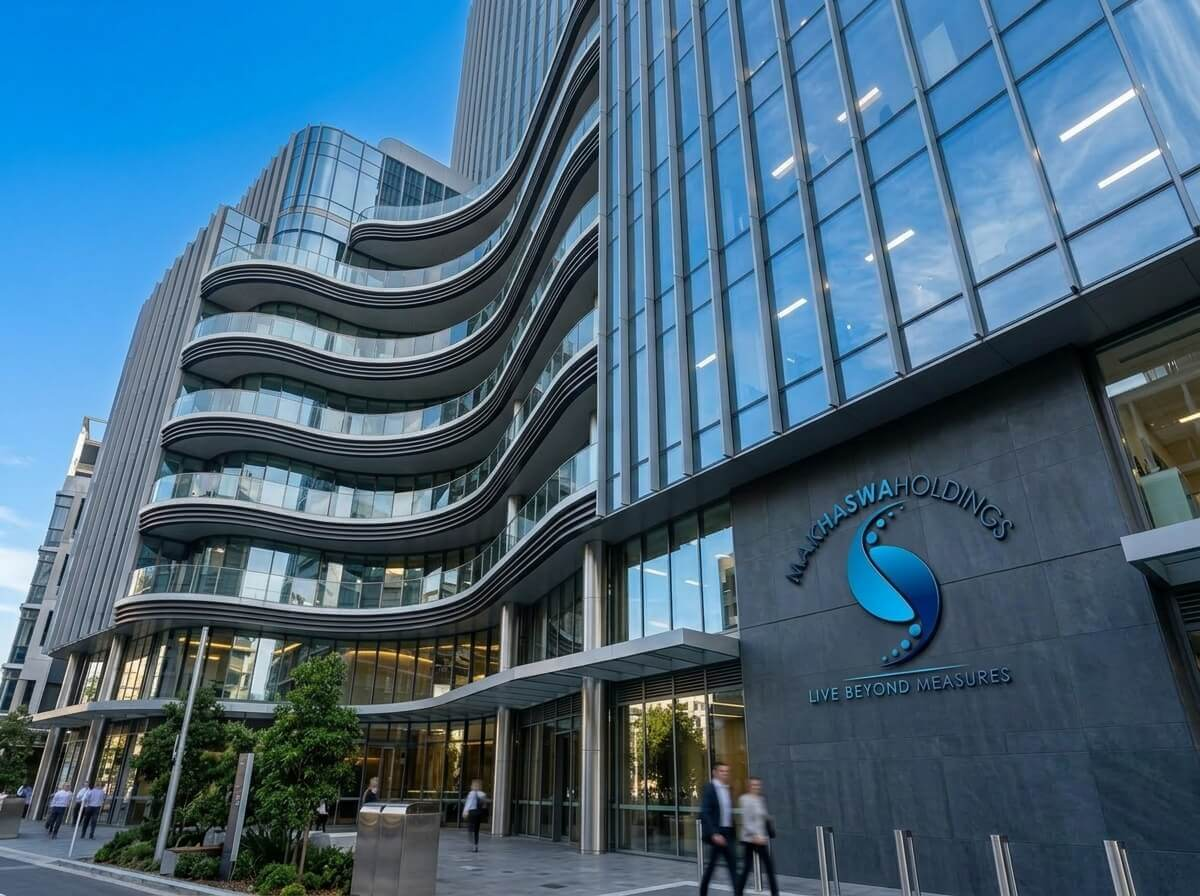
\includegraphics[
                        width=\textwidth,
                        height=5.2cm,
                        keepaspectratio
                    ]{images/makhaswa-building.jpeg}
                \end{tcolorbox}

                \vspace{0.3cm}

                % Key Metrics Quick-Reference Card
                \begin{tcolorbox}[
                    enhanced,
                    colback=mhoffwhite,
                    colframe=mhnavy,
                    boxrule=0.8pt,
                    arc=3pt,
                    title={\bfseries\color{white}\footnotesize Statutory \& Capacity Snapshot},
                    colbacktitle=mhnavy,
                    left=6pt, right=6pt, top=6pt, bottom=6pt
                ]
                    \fontsize{8pt}{11pt}\selectfont
                    \textbf{Company Reg:} K2017/307900/07\\
                    \textbf{CIDB CRS:} 10153817 (Active Grades 8CE/8ME)\\
                    \textbf{B-BBEE Status:} Level 1 (135\% Recognition)\\
                    \textbf{NHBRC Reg:} 4000006217 (Provisional 5)\\
                    \textbf{SARS VAT:} 4840286027 \ $\bullet$ \ \textbf{CSD:} MAAA0584716\\
                    \textbf{COIDA Reg:} 990001157115 \ $\bullet$ \ \textbf{UIF:} 2577464/8
                \end{tcolorbox}

            \end{minipage}
            \hfill
            \begin{minipage}[t]{0.52\textwidth}
                
                {\fontsize{9pt}{12pt}\selectfont\color{mhtextmuted}
                    This profile provides comprehensive evidence of Makhaswa Holdings' legal, technical, financial, and operational readiness to deliver multidisciplinary infrastructure projects.
                }

                \vspace{0.35cm}

                % Styled Table of Contents
                \renewcommand{\arraystretch}{1.35}
                \begin{tabularx}{\textwidth}{@{} X r @{}}
                    \rowcolor{mhoffwhite}
                    {\small\bfseries\color{mhnavy} 01. Executive Overview \& Corporate Identity} & {\small\bfseries\color{mhblue} Page 02} \\
                    {\small\bfseries\color{mhnavy} 02. Strategic Growth Roadmap \& Milestones} & {\small\bfseries\color{mhblue} Page 04} \\
                    \rowcolor{mhoffwhite}
                    {\small\bfseries\color{mhnavy} 03. CIDB Gradings, Accreditations \& Compliance} & {\small\bfseries\color{mhblue} Page 05} \\
                    {\small\bfseries\color{mhnavy} 04. Core Disciplines \& Engineering Capabilities} & {\small\bfseries\color{mhblue} Page 06} \\
                    \rowcolor{mhoffwhite}
                    {\small\bfseries\color{mhnavy} 05. Project Lifecycle \& SHEQ Safety Standards} & {\small\bfseries\color{mhblue} Page 07} \\
                    {\small\bfseries\color{mhnavy} 06. Plant, Heavy Machinery Fleet \& Assets} & {\small\bfseries\color{mhblue} Page 08} \\
                    \rowcolor{mhoffwhite}
                    {\small\bfseries\color{mhnavy} 07. Executive Leadership \& Site Governance} & {\small\bfseries\color{mhblue} Page 09} \\
                    {\small\bfseries\color{mhnavy} 08. Project Portfolio \& Proven Track Record} & {\small\bfseries\color{mhblue} Page 10} \\
                    \rowcolor{mhoffwhite}
                    {\small\bfseries\color{mhnavy} 09. Corporate Social Investment \& Local Upliftment} & {\small\bfseries\color{mhblue} Page 11} \\
                    {\small\bfseries\color{mhnavy} 10. Multi-Provincial Hubs \& Contact Directory} & {\small\bfseries\color{mhblue} Page 12}
                \end{tabularx}

                \vspace{0.4cm}
                \textcolor{mhnavy}{\rule{\textwidth}{0.8pt}}
                \vspace{0.2cm}

                {\fontsize{8pt}{10pt}\selectfont\color{mhtextmuted}Makhaswa Holdings (Pty) Ltd \ $\bullet$ \ Standalone Tender Profile}
            \end{minipage}

        \end{minipage}
    };

\end{tikzpicture}
\clearpage

% =================================================
% PAGE 4 — STRATEGIC TIMELINE & EVOLUTION
% =================================================

\sectionbanner{Company Journey}{Strategic Evolution \& Milestone Track Record}

% Vertical Timeline Card
\begin{tcolorbox}[
    enhanced,
    colback=white,
    colframe=mhlightgray,
    boxrule=0.6pt,
    arc=4pt,
    left=12pt, right=12pt, top=10pt, bottom=10pt,
    drop shadow=black!3
]
    \centering
    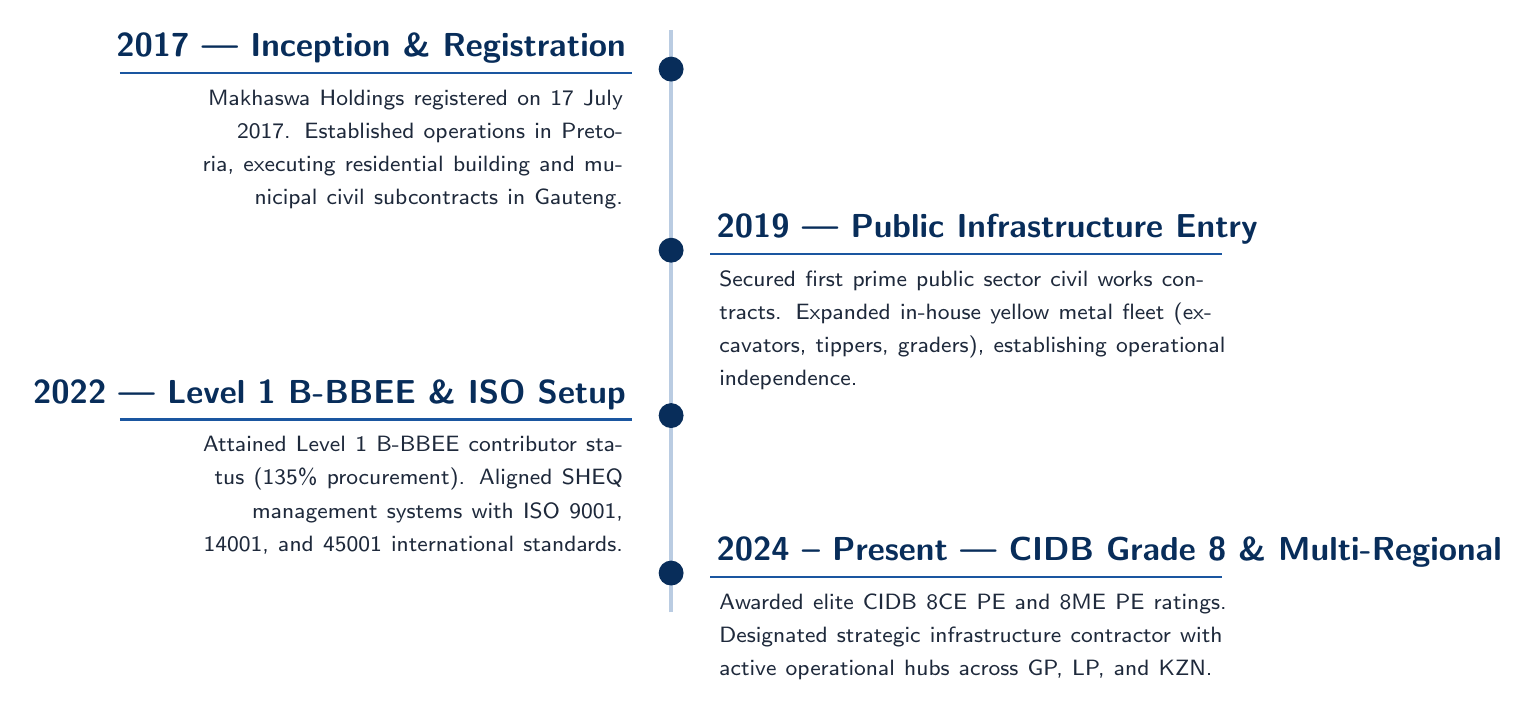
\begin{tikzpicture}[x=1cm, y=1cm]
        % Center Spine Line
        \draw[color=mhblue!30, line width=1.5pt] (0, 0.2) -- (0, 7.6);

        % ----------------------------------------------------
        % 2017 — FOUNDATION
        % ----------------------------------------------------
        \fill[mhnavy] (0, 7.1) circle (4.5pt);
        \node[anchor=south east, inner sep=2pt] at (-0.5, 7.1) {
            {\fontsize{12pt}{14pt}\selectfont\bfseries\color{mhnavy} 2017 — Inception \& Registration}
        };
        \draw[color=mhblue, line width=0.8pt] (-7.0, 7.05) -- (-0.5, 7.05);
        \node[anchor=north east, text width=6.5cm, align=right, inner sep=3pt] at (-0.5, 6.95) {
            {\fontsize{8.2pt}{11pt}\selectfont\color{mhtext} Makhaswa Holdings registered on 17 July 2017. Established operations in Pretoria, executing residential building and municipal civil subcontracts in Gauteng.}
        };

        % ----------------------------------------------------
        % 2019 — PUBLIC SECTOR EXPANSION
        % ----------------------------------------------------
        \fill[mhnavy] (0, 4.8) circle (4.5pt);
        \node[anchor=south west, inner sep=2pt] at (0.5, 4.8) {
            {\fontsize{12pt}{14pt}\selectfont\bfseries\color{mhnavy} 2019 — Public Infrastructure Entry}
        };
        \draw[color=mhblue, line width=0.8pt] (0.5, 4.75) -- (7.0, 4.75);
        \node[anchor=north west, text width=6.5cm, align=left, inner sep=3pt] at (0.5, 4.65) {
            {\fontsize{8.2pt}{11pt}\selectfont\color{mhtext} Secured first prime public sector civil works contracts. Expanded in-house yellow metal fleet (excavators, tippers, graders), establishing operational independence.}
        };

        % ----------------------------------------------------
        % 2022 — TRANSFORMATION & QUALITY ALIGNMENT
        % ----------------------------------------------------
        \fill[mhnavy] (0, 2.7) circle (4.5pt);
        \node[anchor=south east, inner sep=2pt] at (-0.5, 2.7) {
            {\fontsize{12pt}{14pt}\selectfont\bfseries\color{mhnavy} 2022 — Level 1 B-BBEE \& ISO Setup}
        };
        \draw[color=mhblue, line width=0.8pt] (-7.0, 2.65) -- (-0.5, 2.65);
        \node[anchor=north east, text width=6.5cm, align=right, inner sep=3pt] at (-0.5, 2.55) {
            {\fontsize{8.2pt}{11pt}\selectfont\color{mhtext} Attained Level 1 B-BBEE contributor status (135\% procurement). Aligned SHEQ management systems with ISO 9001, 14001, and 45001 international standards.}
        };

        % ----------------------------------------------------
        % 2024 & PRESENT — CIDB GRADE 8 ELEVATION
        % ----------------------------------------------------
        \fill[mhnavy] (0, 0.7) circle (4.5pt);
        \node[anchor=south west, inner sep=2pt] at (0.5, 0.7) {
            {\fontsize{12pt}{14pt}\selectfont\bfseries\color{mhnavy} 2024 -- Present — CIDB Grade 8 \& Multi-Regional}
        };
        \draw[color=mhblue, line width=0.8pt] (0.5, 0.65) -- (7.0, 0.65);
        \node[anchor=north west, text width=6.5cm, align=left, inner sep=3pt] at (0.5, 0.55) {
            {\fontsize{8.2pt}{11pt}\selectfont\color{mhtext} Awarded elite CIDB 8CE PE and 8ME PE ratings. Designated strategic infrastructure contractor with active operational hubs across GP, LP, and KZN.}
        };
    \end{tikzpicture}
\end{tcolorbox}

\vspace{0.25cm}

% Performance Statistics Grid (4 Horizontal Badges)
\noindent
\begin{minipage}{0.235\textwidth}
    \begin{statbadge}
        {\fontsize{16pt}{18pt}\selectfont\bfseries\color{mhnavy} 100+}\\[2pt]
        {\scriptsize\bfseries\color{mhtextmuted} SKILLED WORKFORCE}\\[2pt]
        {\tiny\color{mhtextmuted}Engineers \& Artisans}
    \end{statbadge}
\end{minipage}
\hfill
\begin{minipage}{0.235\textwidth}
    \begin{statbadge}
        {\fontsize{16pt}{18pt}\selectfont\bfseries\color{mhnavy} Level 1}\\[2pt]
        {\scriptsize\bfseries\color{mhtextmuted} B-BBEE STATUS}\\[2pt]
        {\tiny\color{mhtextmuted}135\% Recognition}
    \end{statbadge}
\end{minipage}
\hfill
\begin{minipage}{0.235\textwidth}
    \begin{statbadge}
        {\fontsize{16pt}{18pt}\selectfont\bfseries\color{mhblue} 8 CE PE}\\[2pt]
        {\scriptsize\bfseries\color{mhtextmuted} CIDB GRADING}\\[2pt]
        {\tiny\color{mhtextmuted}Up to R200M Capacity}
    \end{statbadge}
\end{minipage}
\hfill
\begin{minipage}{0.235\textwidth}
    \begin{statbadge}
        {\fontsize{16pt}{18pt}\selectfont\bfseries\color{mhnavy} 4 Hubs}\\[2pt]
        {\scriptsize\bfseries\color{mhtextmuted} PROVINCIAL BASES}\\[2pt]
        {\tiny\color{mhtextmuted}Pretoria, JHB, LP, KZN}
    \end{statbadge}
\end{minipage}

\clearpage

% ===================================================
% PAGE 5 — ACCREDITATIONS & REGULATORY COMPLIANCE
% ===================================================

\sectionbanner{Accreditations}{CIDB CRS 10153817, ISO Standards \& Statutory Mandates}

\noindent
\begin{minipage}[t]{0.485\textwidth}
    
    % CIDB Ratings Breakdown Card
    \begin{brandcard}{CIDB Registration Breakdown}
        \textbf{CRS Number:} 10153817 \ $\bullet$ \ \textbf{Status:} Active\\
        \textbf{Contractor Name:} Makhaswa Holdings (Pty) Ltd

        \vspace{0.25cm}

        \renewcommand{\arraystretch}{1.2}
        \begin{tabularx}{\linewidth}{@{} l X r @{}}
            \rowcolor{mhbluelight}
            \textbf{Grade} & \textbf{Class of Works} & \textbf{Capacity Limit} \\
            \textbf{8CE PE} & Civil Engineering & Up to \textasciitilde R200M \\
            \rowcolor{mhbluelight}
            \textbf{8ME PE} & Mechanical Engineering & Up to \textasciitilde R200M \\
            \textbf{7EB PE} & Electrical Engineering & Up to \textasciitilde R130M \\
            \rowcolor{mhbluelight}
            \textbf{7SB PE} & Specialist Building Works & Up to \textasciitilde R130M \\
            \textbf{6GB PE} & General Building & Up to \textasciitilde R40M
        \end{tabularx}

        \vspace{0.3cm}
        \noindent
        
\includegraphics[width=0.45\textwidth, keepaspectratio]{images/cidb-logo.png}
        \hfill
        \begin{minipage}[b]{0.50\textwidth}
            \fontsize{7.5pt}{10pt}\selectfont\color{mhtextmuted}
            \textit{PE (Potentially Emerging) status empowers Makhaswa to tender on projects one class higher in joint ventures.}
        \end{minipage}
    \end{brandcard}

    \vspace{0.25cm}

    % NHBRC & Quality Accreditations
    \begin{brandcard}{NHBRC Home Builders Registration}
        \textbf{Registration No:} 4000006217\\
        \textbf{Accreditation Status:} Provisional Grade 5\\
        \textbf{Regulatory Act:} Housing Consumers Protection Measures Act

        \vspace{0.2cm}
        
\includegraphics[width=0.75\textwidth, height=1.2cm, keepaspectratio]{images/nhbrc-logo.png}
    \end{brandcard}

\end{minipage}
\hfill
\begin{minipage}[t]{0.485\textwidth}
    
    % ISO Certifications Card
    \begin{brandcard}{International ISO Standards Compliance}
        Fully implemented Integrated Management System (IMS) guaranteeing global best practices:

        \begin{itemize}[leftmargin=12pt, itemsep=3pt, label=\color{mhblue}$\blacktriangleright$]
            \item \textbf{ISO 9001:2015} \ Quality Management System (QMS)
            \item \textbf{ISO 14001:2015} \ Environmental Management System (EMS)
            \item \textbf{ISO 45001:2018} \ Occupational Health \& Safety (OH\&S)
        \end{itemize}

        \vspace{0.15cm}
        \noindent
        
\includegraphics[width=0.38\textwidth, keepaspectratio]{images/iso-logo.png}
        \hfill
        
\includegraphics[width=0.38\textwidth, keepaspectratio]{images/sheq-logo.png}
    \end{brandcard}

    \vspace{0.25cm}

    % Corporate Statutory & Tax Verification
    \begin{brandcard}{Corporate Compliance \& Tax Status}
        \begin{itemize}[leftmargin=12pt, itemsep=2.5pt, label=\color{mhblue}$\blacktriangleright$]
            \item \textbf{B-BBEE Rating:} Level 1 (135\% Procurement Level)
            \item \textbf{Ownership:} 100\% Black Owned Enterprise
            \item \textbf{National Treasury CSD:} MAAA0584716
            \item \textbf{SARS VAT Number:} 4840286027
            \item \textbf{COIDA Compensation:} Reg No: 990001157115
            \item \textbf{Department of Labour UIF:} Reg No: 2577464/8
        \end{itemize}

        \vspace{0.2cm}
        \noindent
        
\includegraphics[width=0.42\textwidth, keepaspectratio]{images/bbbee-logo.png}
        \hfill
        \begin{minipage}[b]{0.52\textwidth}
            \fontsize{7.5pt}{10pt}\selectfont\color{mhnavy}\bfseries
            Good Standing with SARS, Department of Labour \& Compensation Fund.
        \end{minipage}
    \end{brandcard}

\end{minipage}

\clearpage

% ===================================================
% PAGE 6 — CORE DISCIPLINES & CAPABILITIES
% ===================================================

\sectionbanner{Capabilities}{Full-Spectrum Engineering \& Infrastructure Execution}

% Top 3 Discipline Cards
\noindent
\begin{minipage}[t]{0.31\textwidth}
    \begin{darkservice}
        \textbf{\normalsize 01. Earthworks \& Civils}\\[3pt]
        \fontsize{8pt}{11pt}\selectfont
        Site clearance, mass cut/fill earthworks, platform preparation, stormwater retention, and deep trenching.
    \end{darkservice}
\end{minipage}
\hfill
\begin{minipage}[t]{0.31\textwidth}
    \begin{darkservice}
        \textbf{\normalsize 02. Roads \& Surfacing}\\[3pt]
        \fontsize{8pt}{11pt}\selectfont
        Subbase layer works, asphalt paving (overlays/inlays), kerbing, concrete stabilization, and road markings.
    \end{darkservice}
\end{minipage}
\hfill
\begin{minipage}[t]{0.31\textwidth}
    \begin{darkservice}
        \textbf{\normalsize 03. Building \& MEP}\\[3pt]
        \fontsize{8pt}{11pt}\selectfont
        Commercial buildings, pump station piping, HVAC systems, and high-mast electrical infrastructure.
    \end{darkservice}
\end{minipage}

\vspace{0.4cm}

% Detailed Scope Matrix + Visual Grid
\noindent
\begin{minipage}[t]{0.43\textwidth}
    {\large\bfseries\color{mhnavy} CORE DELIVERABLES}
    \vspace{0.2cm}

    \begin{itemize}[leftmargin=10pt, itemsep=4pt, label=\color{mhnavy}$\blacksquare$]
        \item \textbf{Mass Earthworks:} Site leveling, rock excavation, spoil removal, and platform preparation.
        \item \textbf{Civil Stormwater:} Culvert installation, sewer lines, stone pitching, gabions, and Reno mattresses.
        \item \textbf{Road Infrastructure:} Layer works, asphalt profiling, paving, kerbing, and guardrails.
        \item \textbf{Structural Building:} Commercial structures, residential housing schemes, and industrial warehouses.
        \item \textbf{Mechanical Systems:} Pumphouses, heavy steel piping, valve chambers, and HVAC.
        \item \textbf{Electrical Networks:} High-mast lighting, substations, and power reticulation.
    \end{itemize}
\end{minipage}
\hfill
\begin{minipage}[t]{0.54\textwidth}
    {\large\bfseries\color{mhnavy} PROVEN SITE DEPLOYMENTS}
    \vspace{0.2cm}

    % Image Grid (2 Rows x 3 Columns)
    \noindent
    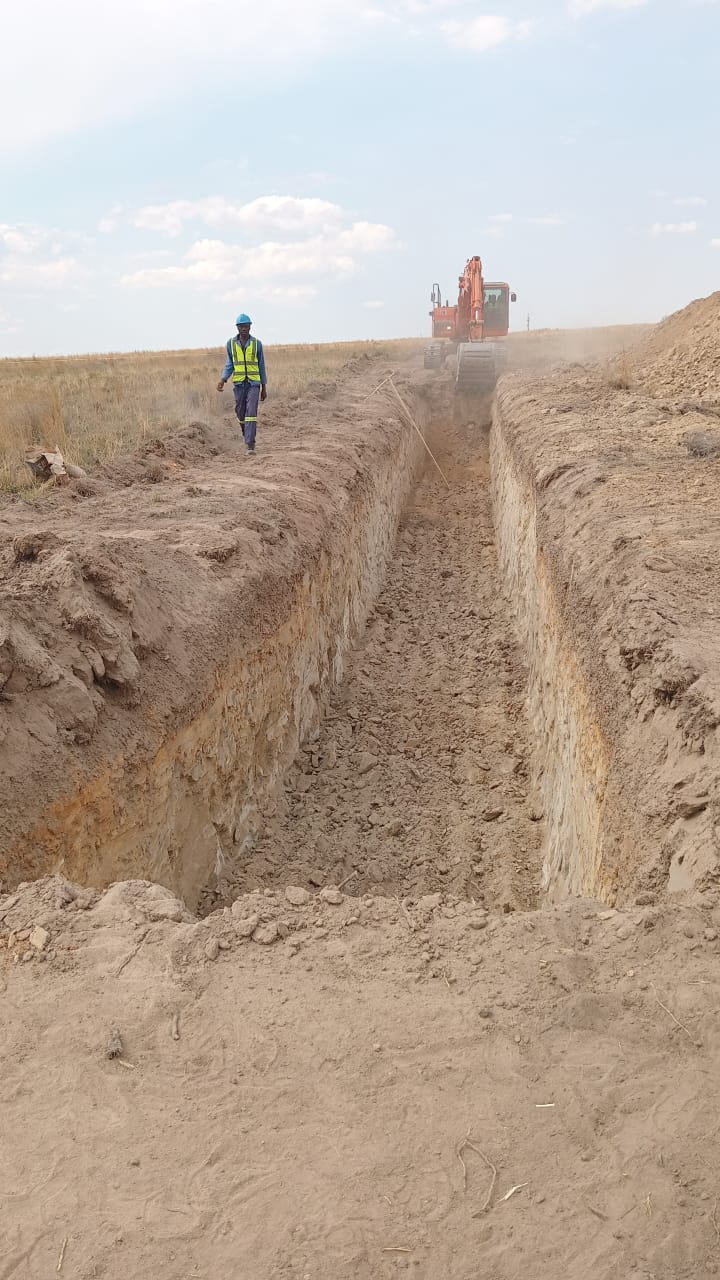
\includegraphics[width=0.31\textwidth, height=2.2cm]{images/bulk-trenching-earthworks-1.jpeg}
    \hfill
    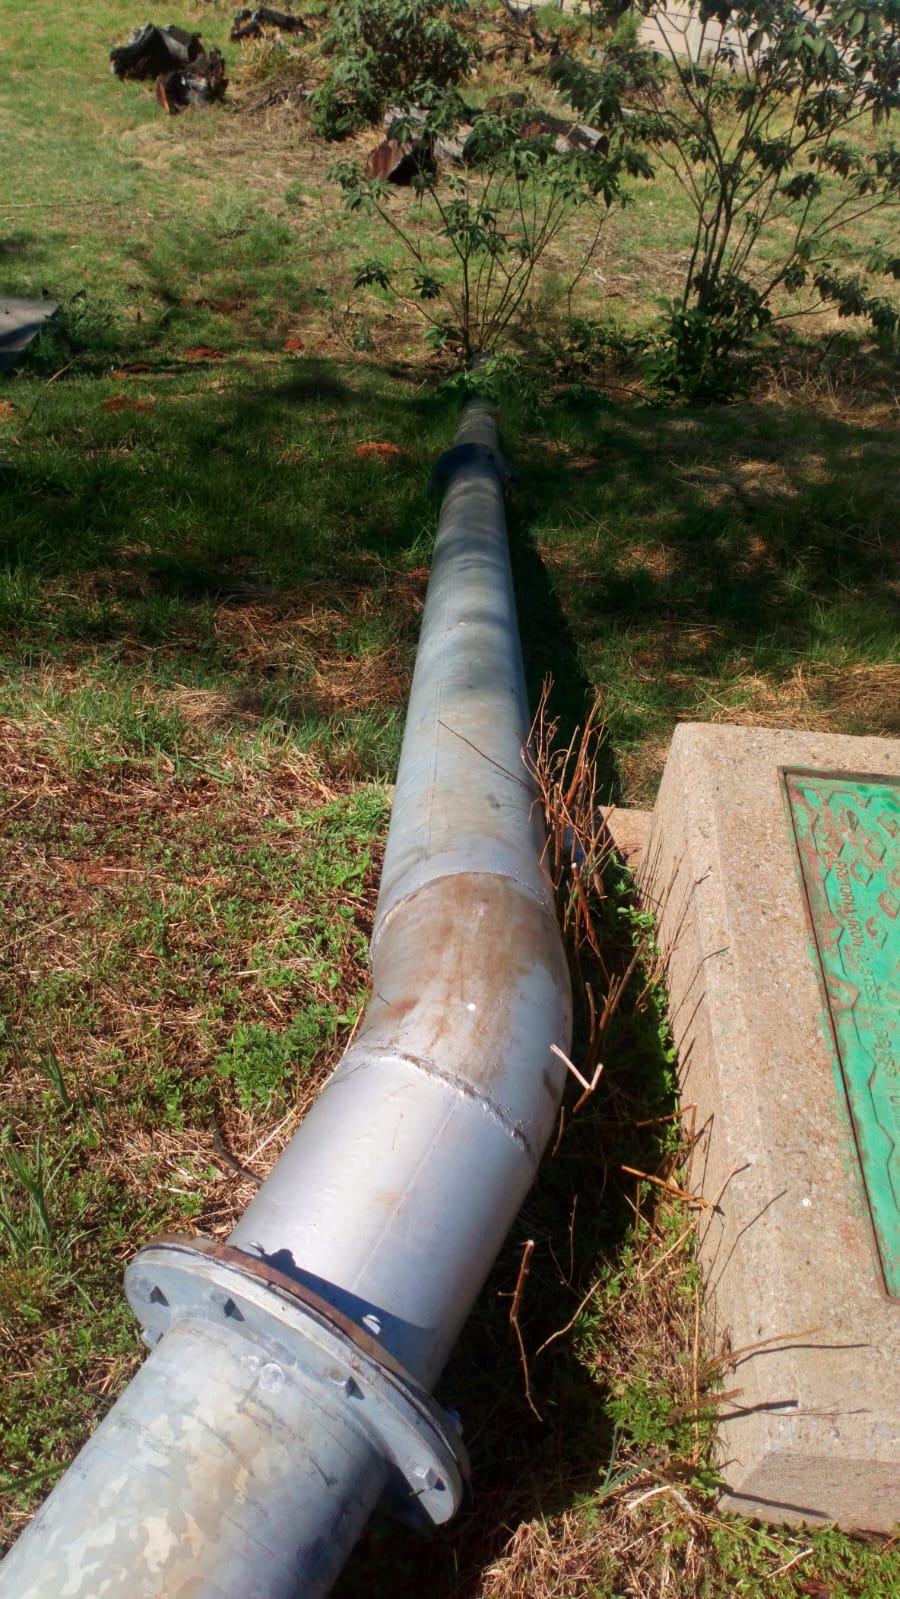
\includegraphics[width=0.31\textwidth, height=2.2cm]{images/pumphouse-steel-pipe-works-2.jpeg}
    \hfill
    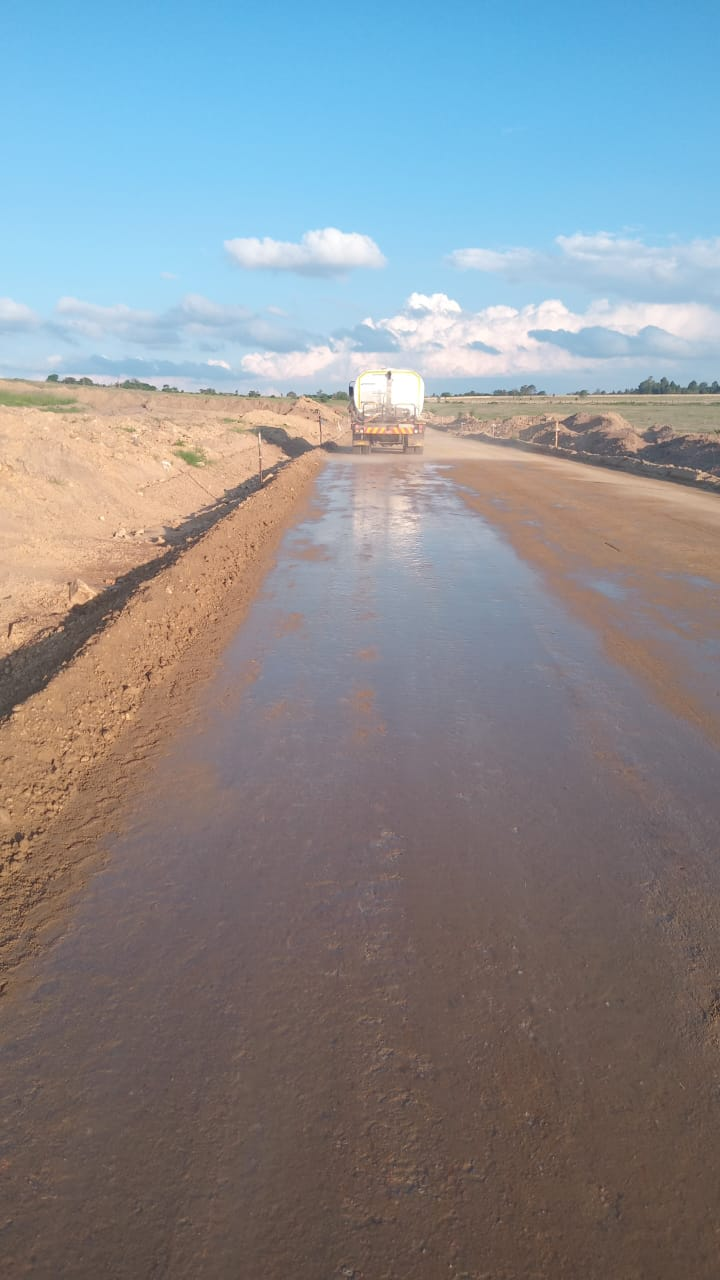
\includegraphics[width=0.31\textwidth, height=2.2cm]{images/earthworks-surfacing-1.jpeg}

    \vspace{0.15cm}

    \noindent
    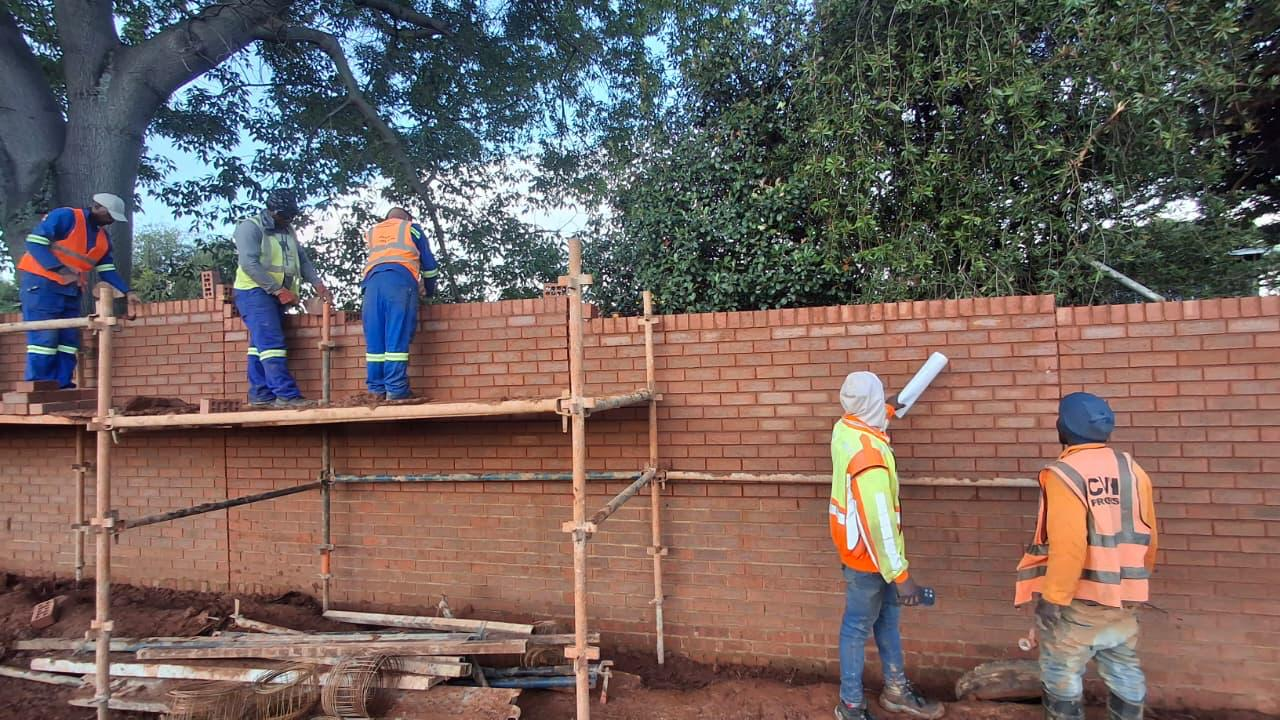
\includegraphics[width=0.31\textwidth, height=2.2cm]{images/makhaswa (21).jpeg}
    \hfill
    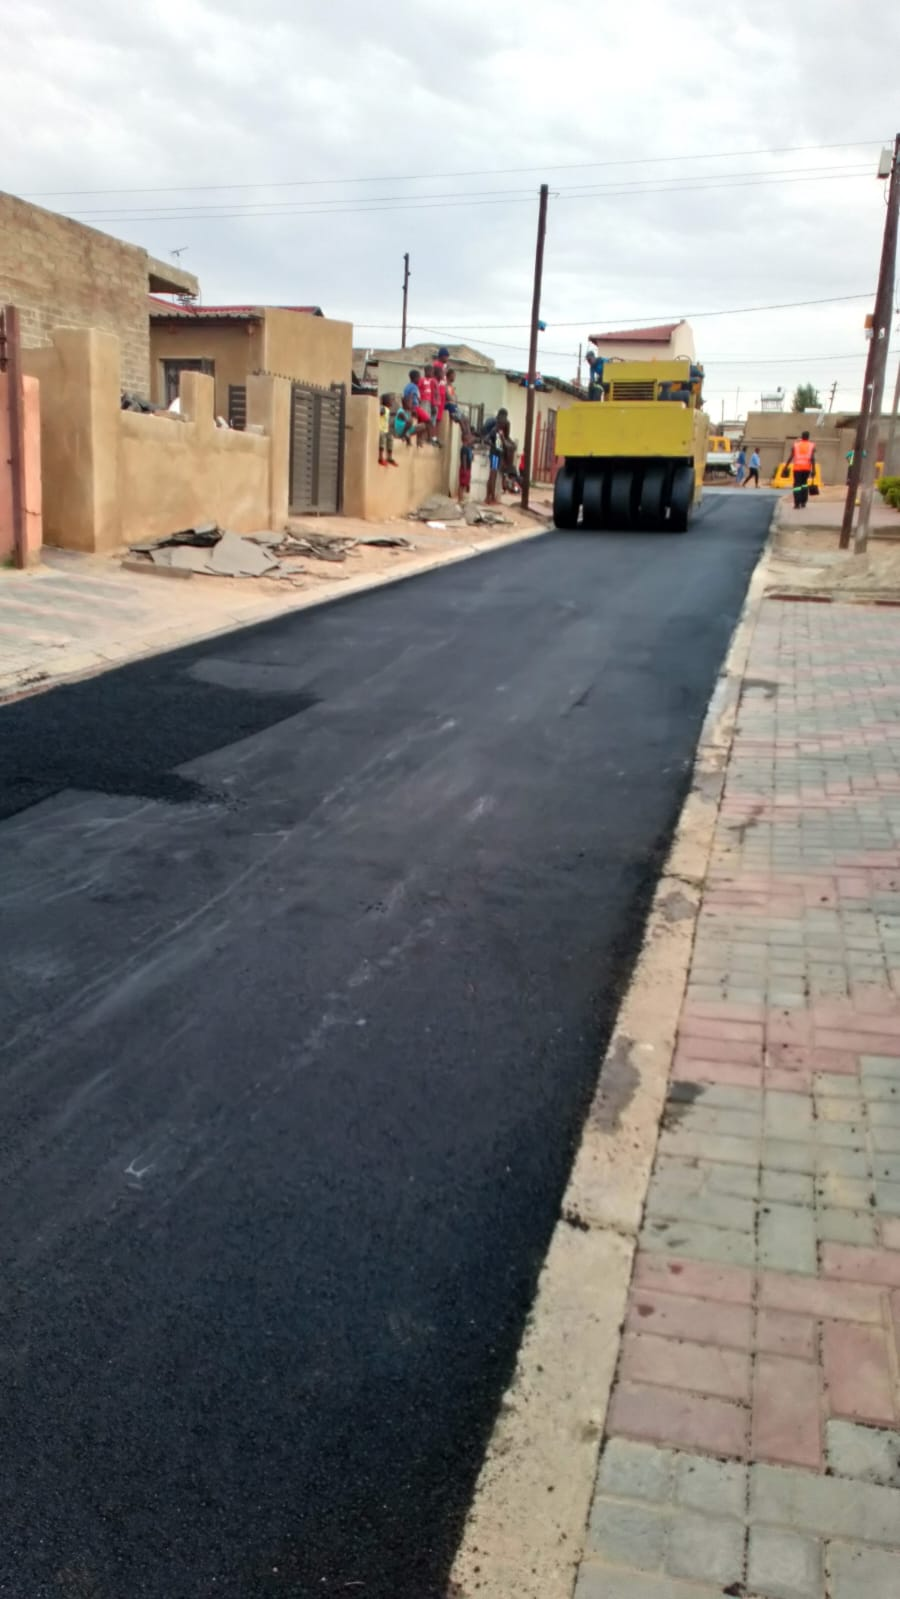
\includegraphics[width=0.31\textwidth, height=2.2cm]{images/asphalt-photos-1.jpeg}
    \hfill
    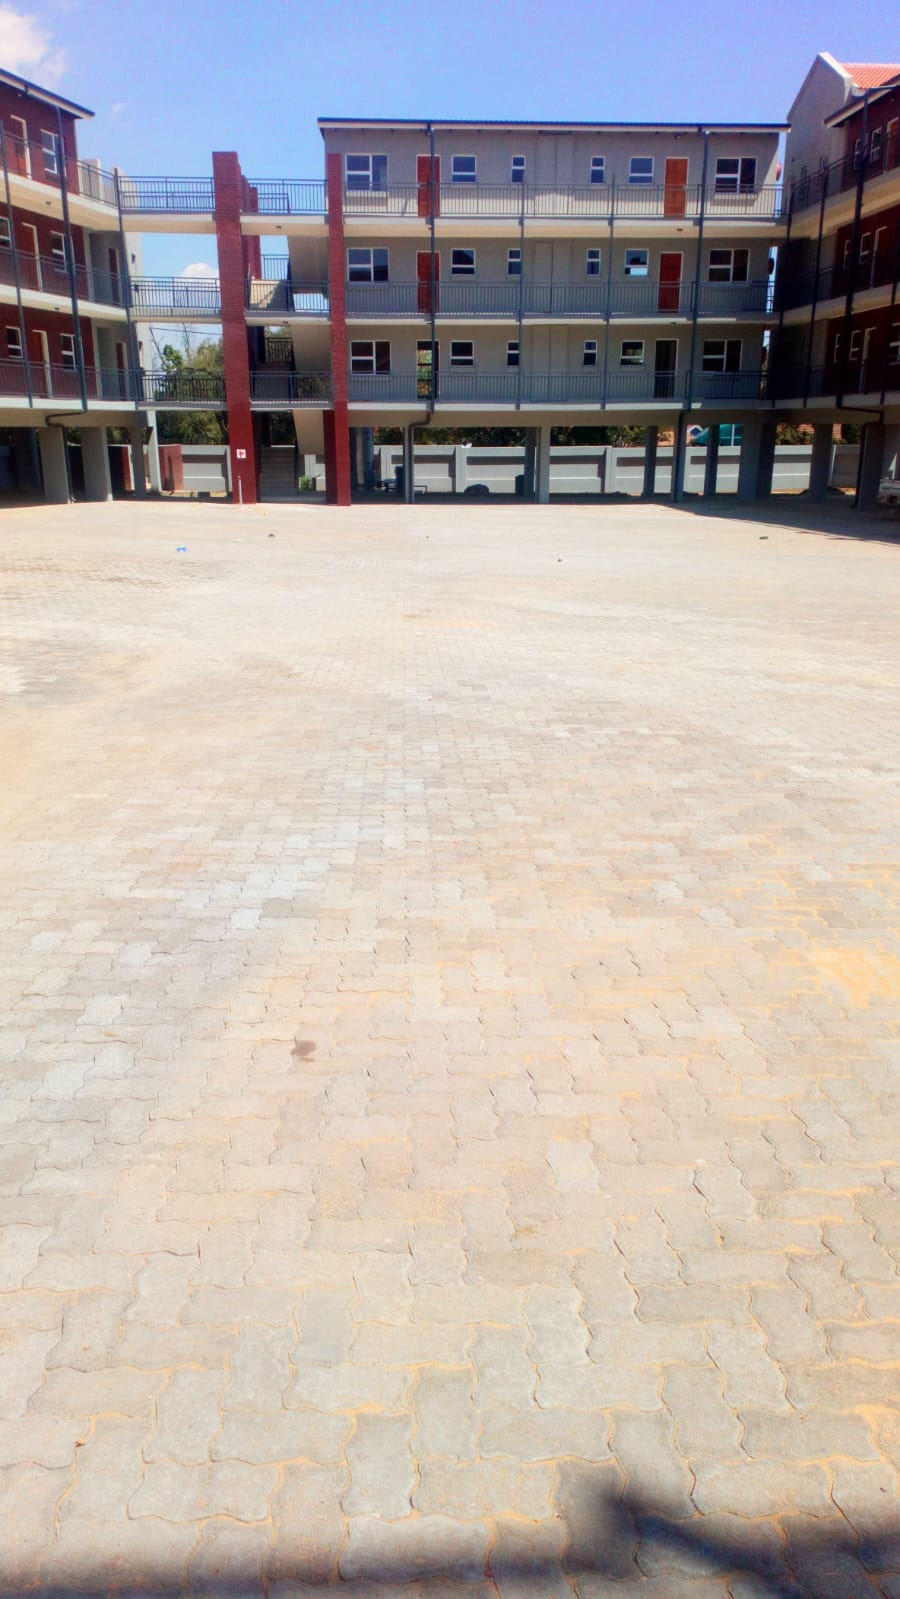
\includegraphics[width=0.31\textwidth, height=2.2cm]{images/building-photos-1.jpeg}
\end{minipage}

\vspace{0.35cm}

% Project Management Methodology Note
\begin{tcolorbox}[
    enhanced,
    colback=mhoffwhite,
    colframe=mhlightgray,
    boxrule=0.7pt,
    arc=3pt,
    left=10pt, right=10pt, top=8pt, bottom=8pt,
    borderline west={3pt}{0pt}{mhnavy}
]
    \fontsize{8.5pt}{12pt}\selectfont\color{mhtext}
    \textbf{Turnkey Management:} From preliminary feasibility and geotechnical surveying to structural execution and statutory closeout, Makhaswa Holdings coordinates all trades with precision project controls and budget discipline.
\end{tcolorbox}

\clearpage

% ===================================================
% PAGE 7 — PROJECT LIFECYCLE & SHEQ SAFETY FRAMEWORK
% ===================================================

\sectionbanner{Delivery \& SHEQ}{4-Stage Project Lifecycle \& Safety Management}

% 4-Stage Lifecycle Horizontal Workflow
\noindent
\begin{minipage}[t]{0.235\textwidth}
    \begin{tcolorbox}[
        enhanced, colback=mhnavy, colframe=mhnavy, boxrule=0pt, arc=3pt,
        coltext=white, left=6pt, right=6pt, top=8pt, bottom=8pt, height=3.6cm
    ]
        {\small\bfseries\color{mhbluelight} STAGE 01}\\
        {\footnotesize\bfseries Feasibility \& Design}\\[0.15cm]
        \fontsize{7.5pt}{10.5pt}\selectfont
        Site survey, geotechnical analysis, bill of quantities review, constructability assessments, and risk registers.
    \end{tcolorbox}
\end{minipage}
\hfill
\begin{minipage}[t]{0.235\textwidth}
    \begin{tcolorbox}[
        enhanced, colback=mhnavy2, colframe=mhnavy2, boxrule=0pt, arc=3pt,
        coltext=white, left=6pt, right=6pt, top=8pt, bottom=8pt, height=3.6cm
    ]
        {\small\bfseries\color{mhbluelight} STAGE 02}\\
        {\footnotesize\bfseries Planning \& Sourcing}\\[0.15cm]
        \fontsize{7.5pt}{10.5pt}\selectfont
        Project baseline schedule, procurement of SABS materials, plant deployment, and local community liaison setup.
    \end{tcolorbox}
\end{minipage}
\hfill
\begin{minipage}[t]{0.235\textwidth}
    \begin{tcolorbox}[
        enhanced, colback=mhnavy3, colframe=mhnavy3, boxrule=0pt, arc=3pt,
        coltext=white, left=6pt, right=6pt, top=8pt, bottom=8pt, height=3.6cm
    ]
        {\small\bfseries\color{white} STAGE 03}\\
        {\footnotesize\bfseries Site Execution}\\[0.15cm]
        \fontsize{7.5pt}{10.5pt}\selectfont
        Direct on-site management, continuous QA/QC compaction/concrete testing, daily toolbox talks, and milestone delivery.
    \end{tcolorbox}
\end{minipage}
\hfill
\begin{minipage}[t]{0.235\textwidth}
    \begin{tcolorbox}[
        enhanced, colback=mhnavy, colframe=mhnavy, boxrule=0pt, arc=3pt,
        coltext=white, left=6pt, right=6pt, top=8pt, bottom=8pt, height=3.6cm
    ]
        {\small\bfseries\color{mhbluelight} STAGE 04}\\
        {\footnotesize\bfseries Closeout \& Handover}\\[0.15cm]
        \fontsize{7.5pt}{10.5pt}\selectfont
        As-built documentation, engineer sign-offs, municipal compliance certifications, defects liability, and client handover.
    \end{tcolorbox}
\end{minipage}

\vspace{0.5cm}

% Detailed SHEQ Policy (Left) & Quality Assurance (Right)
\noindent
\begin{minipage}[t]{0.485\textwidth}
    \begin{brandcard}{Safety, Health \& Environmental (SHEQ)}
        Makhaswa maintains a strict \textbf{Zero-Harm Policy} governed by the Occupational Health and Safety Act (Act 85 of 1993):

        \begin{itemize}[leftmargin=12pt, itemsep=3.5pt, label=\color{mhblue}$\blacktriangleright$]
            \item \textbf{SACPCMP-Registered Officers:} Full-time SHEQ officers on every active site.
            \item \textbf{Daily Safety Audits:} Pre-task risk assessments (HIRA) and compulsory daily toolbox talks.
            \item \textbf{PPE Compliance:} Strict enforcement of certified Personal Protective Equipment across all trades.
            \item \textbf{Environmental Care:} Soil conservation, spill prevention, and eco-friendly waste management.
        \end{itemize}
    \end{brandcard}
\end{minipage}
\hfill
\begin{minipage}[t]{0.485\textwidth}
    \begin{brandcard}{Quality Assurance \& Material Standards}
        Uncompromising quality controls to ensure long-term structural durability:

        \begin{itemize}[leftmargin=12pt, itemsep=3.5pt, label=\color{mhblue}$\blacktriangleright$]
            \item \textbf{SABS/SANAS Certified Materials:} Only tested and approved aggregate, asphalt, and steel.
            \item \textbf{Compaction \& Slump Tests:} Routine laboratory testing of soil density and concrete compressive strength.
            \item \textbf{Surveyor Verification:} Land surveying with digital total stations and GPS for precise elevation and grading.
            \item \textbf{Defect-Free Guarantee:} Continuous quality inspections prior to milestone certifications.
        \end{itemize}
    \end{brandcard}
\end{minipage}

\clearpage

% ===================================================
% PAGE 8 — PLANT, MACHINERY FLEET & ASSETS
% ===================================================

\sectionbanner{Plant \& Fleet}{In-House Heavy Machinery \& Technical Assets}

\noindent
{\fontsize{9.5pt}{13.5pt}\selectfont\color{mhtext}
    To ensure project momentum, eliminate reliance on third-party hire delays, and guarantee rapid site mobilization, Makhaswa Holdings owns and operates an extensive yellow metal, road-building, and transport fleet:
}

\vspace{0.35cm}

% Machinery Categories (4 Feature Cards)
\noindent
\begin{minipage}[t]{0.485\textwidth}
    \begin{brandcard}{Earthmoving \& Excavation Equipment}
        \begin{itemize}[leftmargin=12pt, itemsep=3pt, label=\color{mhblue}$\blacktriangleright$]
            \item \textbf{Tracked Excavators (20T -- 30T):} Heavy bulk trenching, rock breaking, and site clearance.
            \item \textbf{Articulated Dump Trucks (ADTs):} High-volume mass earthmoving and spoil hauling.
            \item \textbf{TLBs (4x4 Tractor Loaders):} Agile trenching, pipe-laying, and site loading.
            \item \textbf{Skid Steer Loaders (Bobcats):} Confined space excavation and cleanup.
        \end{itemize}
    \end{brandcard}

    \vspace{0.25cm}

    \begin{brandcard}{Road Construction \& Surfacing Plant}
        \begin{itemize}[leftmargin=12pt, itemsep=3pt, label=\color{mhblue}$\blacktriangleright$]
            \item \textbf{Motor Graders (CAT 140K/G):} Subbase leveling, profiling, and road cambering.
            \item \textbf{Smooth Drum \& Padfoot Rollers (10T -- 12T):} Soil and layer-work compaction.
            \item \textbf{Pneumatic Tyre Rollers (PTR):} Asphalt compaction and seal finishing.
            \item \textbf{Asphalt Pavers \& Chip Spreaders:} Precision surfacing.
        \end{itemize}
    \end{brandcard}
\end{minipage}
\hfill
\begin{minipage}[t]{0.485\textwidth}
    \begin{brandcard}{Haulage, Logistics \& Utility Fleet}
        \begin{itemize}[leftmargin=12pt, itemsep=3pt, label=\color{mhblue}$\blacktriangleright$]
            \item \textbf{Tipper Trucks (10m$^3$ -- 15m$^3$):} Aggregate, asphalt, and material delivery.
            \item \textbf{Water Bowsers (10,000L -- 16,000L):} Compaction moisture control and dust suppression.
            \item \textbf{Lowbed Transport Trailers:} Heavy machinery mobilization across provinces.
            \item \textbf{Site Support Vehicles (4x4 LDVs):} Engineering and supervisory mobility.
        \end{itemize}
    \end{brandcard}

    \vspace{0.25cm}

    \begin{brandcard}{Surveying \& Specialist Technical Assets}
        \begin{itemize}[leftmargin=12pt, itemsep=3pt, label=\color{mhblue}$\blacktriangleright$]
            \item \textbf{Digital Total Stations \& Optical Levels:} Micro-accuracy surveying.
            \item \textbf{Differential GPS Rovers:} Real-time road profiling and topography.
            \item \textbf{Concrete Batching \& Core Drilling Equipment.}
            \item \textbf{Mobile Diesel Generators \& Lighting Towers.}
        \end{itemize}
    \end{brandcard}
\end{minipage}

\vspace{0.35cm}

% Maintenance & Reliability Note
\begin{tcolorbox}[
    enhanced,
    colback=mhnavy,
    colframe=mhnavy,
    boxrule=0pt,
    arc=3pt,
    left=10pt, right=10pt, top=8pt, bottom=8pt,
    halign=center
]
    \color{white}
    \fontsize{8.5pt}{12pt}\selectfont
    \textbf{Fleet Reliability Guarantee:} All equipment undergoes scheduled mechanical servicing by qualified technicians, ensuring maximum on-site uptime, operator safety, and zero project delays.
\end{tcolorbox}

\clearpage

% ===================================================
% PAGE 9 — EXECUTIVE LEADERSHIP & KEY PERSONNEL
% ===================================================

\sectionbanner{Leadership}{Executive Management \& Site Governance}

\noindent
{\fontsize{9.5pt}{13.5pt}\selectfont\color{mhtext}
    Makhaswa Holdings is spearheaded by a dynamic team of professionally registered engineers, project managers, and seasoned construction leaders dedicated to engineering excellence:
}

\vspace{0.4cm}

% 6 Leadership Cards (2 Columns x 3 Rows)
\noindent
\begin{minipage}[t]{0.485\textwidth}
    \begin{featurecard}{Lucas Dinga}
        \textbf{Chief Executive Officer (CEO)}\\
        \fontsize{8pt}{11pt}\selectfont\color{mhtextmuted}
        Visionary executive leading strategic corporate expansion, tender governance, public-private partnerships, and operational delivery across South Africa.
    \end{featurecard}

    \vspace{0.2cm}

    \begin{featurecard}{Lindelani Shangase}
        \textbf{SHEQ Officer (Pr.OHS)}\\
        \fontsize{8pt}{11pt}\selectfont\color{mhtextmuted}
        Certified occupational safety professional overseeing zero-harm compliance, environmental protection protocols, and ISO management systems.
    \end{featurecard}

    \vspace{0.2cm}

    \begin{featurecard}{Hendrick Chauke}
        \textbf{Quality Controller (QA/QC)}\\
        \fontsize{8pt}{11pt}\selectfont\color{mhtextmuted}
        Technical quality controller managing material testing, compaction density verification, concrete crush tests, and defect-free handover.
    \end{featurecard}
\end{minipage}
\hfill
\begin{minipage}[t]{0.485\textwidth}
    \begin{featurecard}{Sfiso Nkabinde}
        \textbf{Construction Manager / Senior Site Agent}\\
        \fontsize{8pt}{11pt}\selectfont\color{mhtextmuted}
        Seasoned civil engineer managing large-scale earthworks, road construction, plant deployment, site logistics, and critical-path scheduling.
    \end{featurecard}

    \vspace{0.2cm}

    \begin{featurecard}{Henry Chauke}
        \textbf{Section Supervisor}\\
        \fontsize{8pt}{11pt}\selectfont\color{mhtextmuted}
        Field operations supervisor directing specialized civil trades, trenching safety, structural concrete, and daily site productivity.
    \end{featurecard}

    \vspace{0.2cm}

    \begin{featurecard}{C. Mazarura}
        \textbf{Professional Land Surveyor}\\
        \fontsize{8pt}{11pt}\selectfont\color{mhtextmuted}
        Expert surveyor utilizing high-precision GPS and Total Station instruments for road profiling, earthworks calculations, and setting out.
    \end{featurecard}
\end{minipage}

\vspace{0.45cm}

% Human Capital Capacity Box
\begin{tcolorbox}[
    enhanced,
    colback=mhoffwhite,
    colframe=mhnavy,
    boxrule=0.8pt,
    arc=4pt,
    left=10pt, right=10pt, top=10pt, bottom=10pt,
    title={\bfseries\color{white}\small Multi-Disciplinary Human Capital},
    colbacktitle=mhnavy
]
    \fontsize{8.5pt}{12pt}\selectfont\color{mhtext}
    Our permanent core staff is supported by a scalable pool of over \textbf{100 to 200 skilled artisans}, machine operators, pipe-fitters, pavers, steel-fixers, and local general workers. We prioritize continuous technical training, trade apprenticeships, and on-site skills development.
\end{tcolorbox}

\clearpage

% ===================================================
% PAGE 10 — FEATURED PROJECT PORTFOLIO & TRACK RECORD
% ===================================================

\sectionbanner{Portfolio}{Selected Civil, Road \& Infrastructure Deployments}

\noindent
% Row 1 of Projects
\begin{minipage}[t]{0.315\textwidth}
    \begin{tcolorbox}[enhanced, colback=white, colframe=mhlightgray, boxrule=0.7pt, arc=3pt, left=0pt, right=0pt, top=0pt, bottom=6pt]
        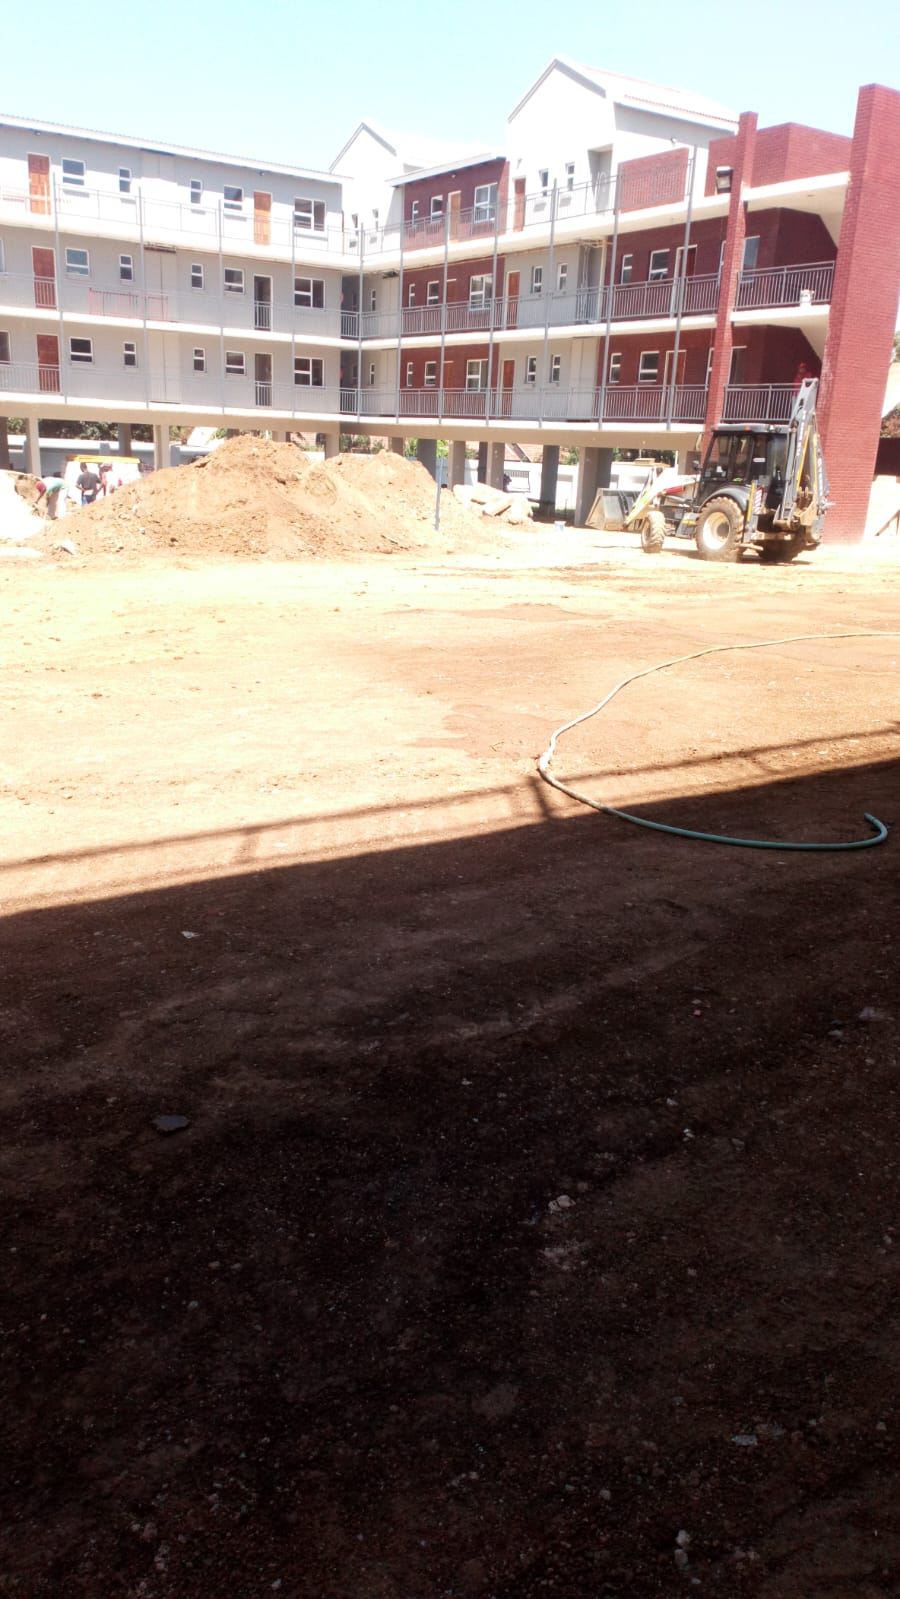
\includegraphics[width=\textwidth, height=3.4cm]{images/building-photos-6.jpeg}
        \vspace{2pt}
        \centering
        {\scriptsize\bfseries\color{mhtextmuted} GENERAL BUILDING}\\
        {\footnotesize\bfseries\color{mhnavy} Structural Masonry \& Walls}
    \end{tcolorbox}
\end{minipage}
\hfill
\begin{minipage}[t]{0.315\textwidth}
    \begin{tcolorbox}[enhanced, colback=white, colframe=mhlightgray, boxrule=0.7pt, arc=3pt, left=0pt, right=0pt, top=0pt, bottom=6pt]
        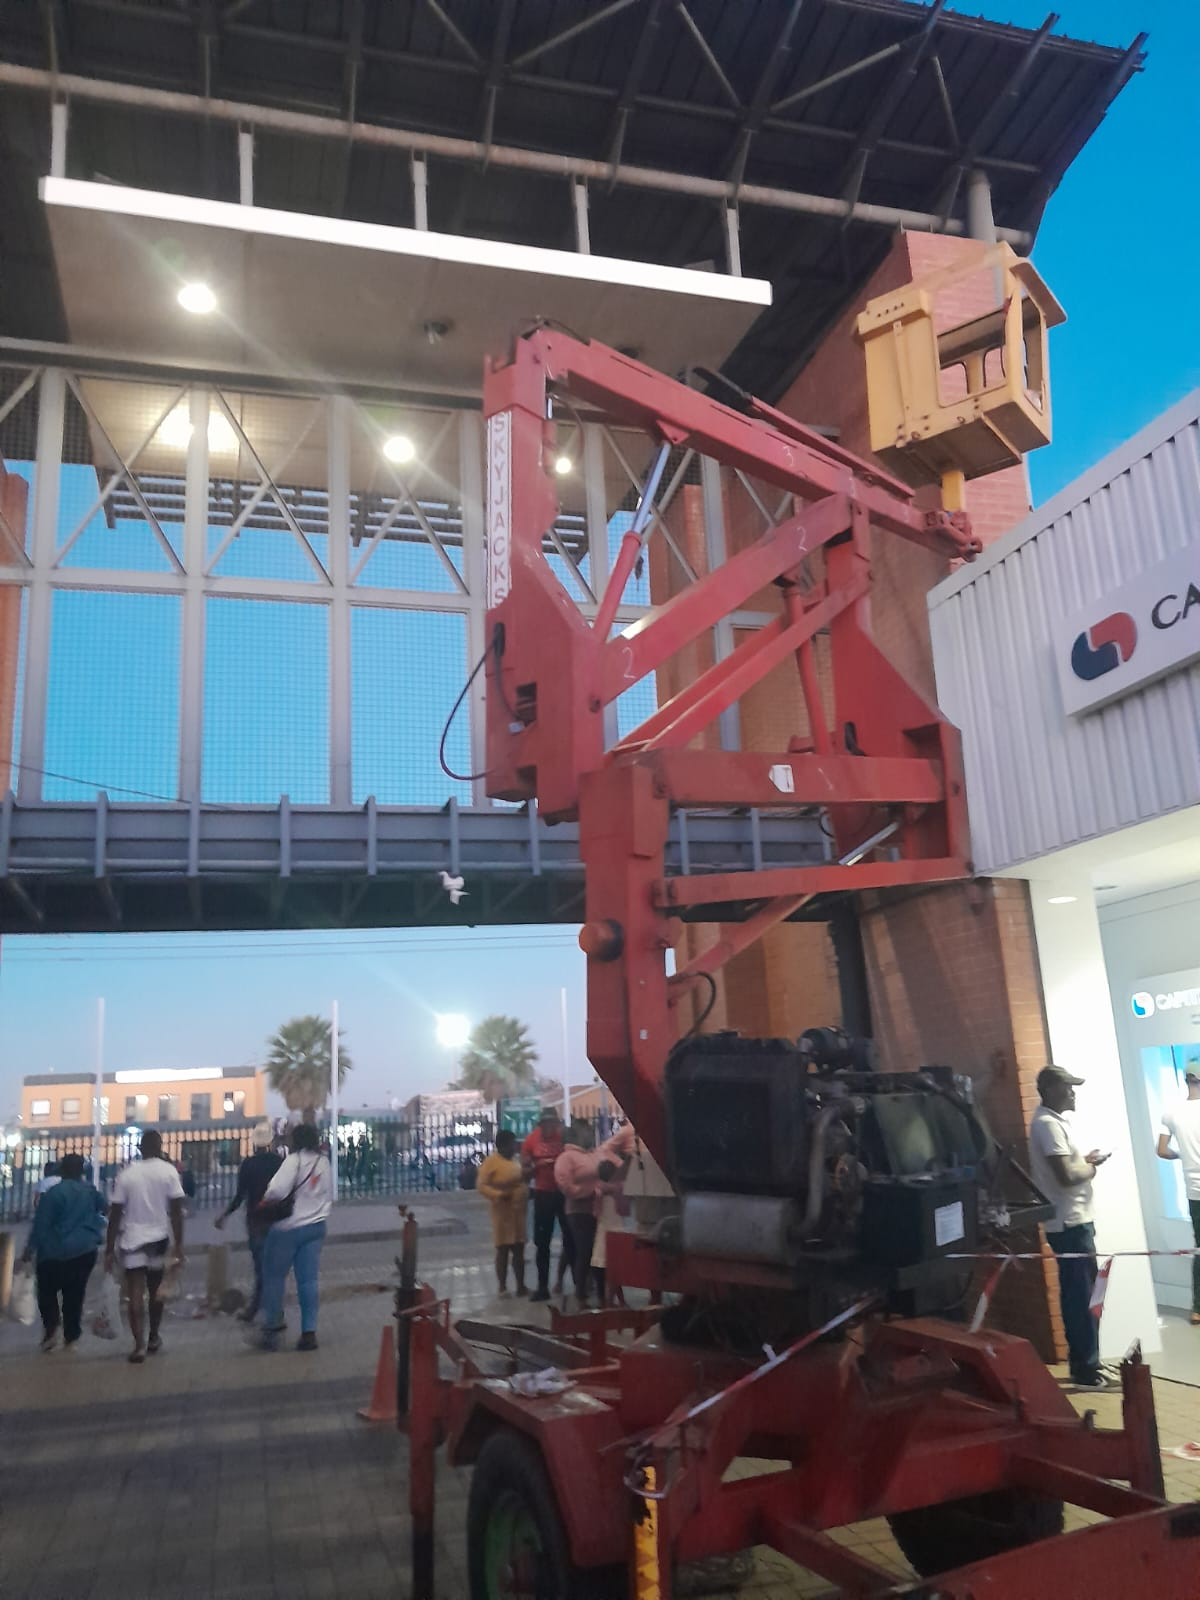
\includegraphics[width=\textwidth, height=3.4cm]{images/high-mast-electrical-1.jpeg}
        \vspace{2pt}
        \centering
        {\scriptsize\bfseries\color{mhtextmuted} ELECTRICAL RETICULATION}\\
        {\footnotesize\bfseries\color{mhnavy} High-Mast Lighting Systems}
    \end{tcolorbox}
\end{minipage}
\hfill
\begin{minipage}[t]{0.315\textwidth}
    \begin{tcolorbox}[enhanced, colback=white, colframe=mhlightgray, boxrule=0.7pt, arc=3pt, left=0pt, right=0pt, top=0pt, bottom=6pt]
        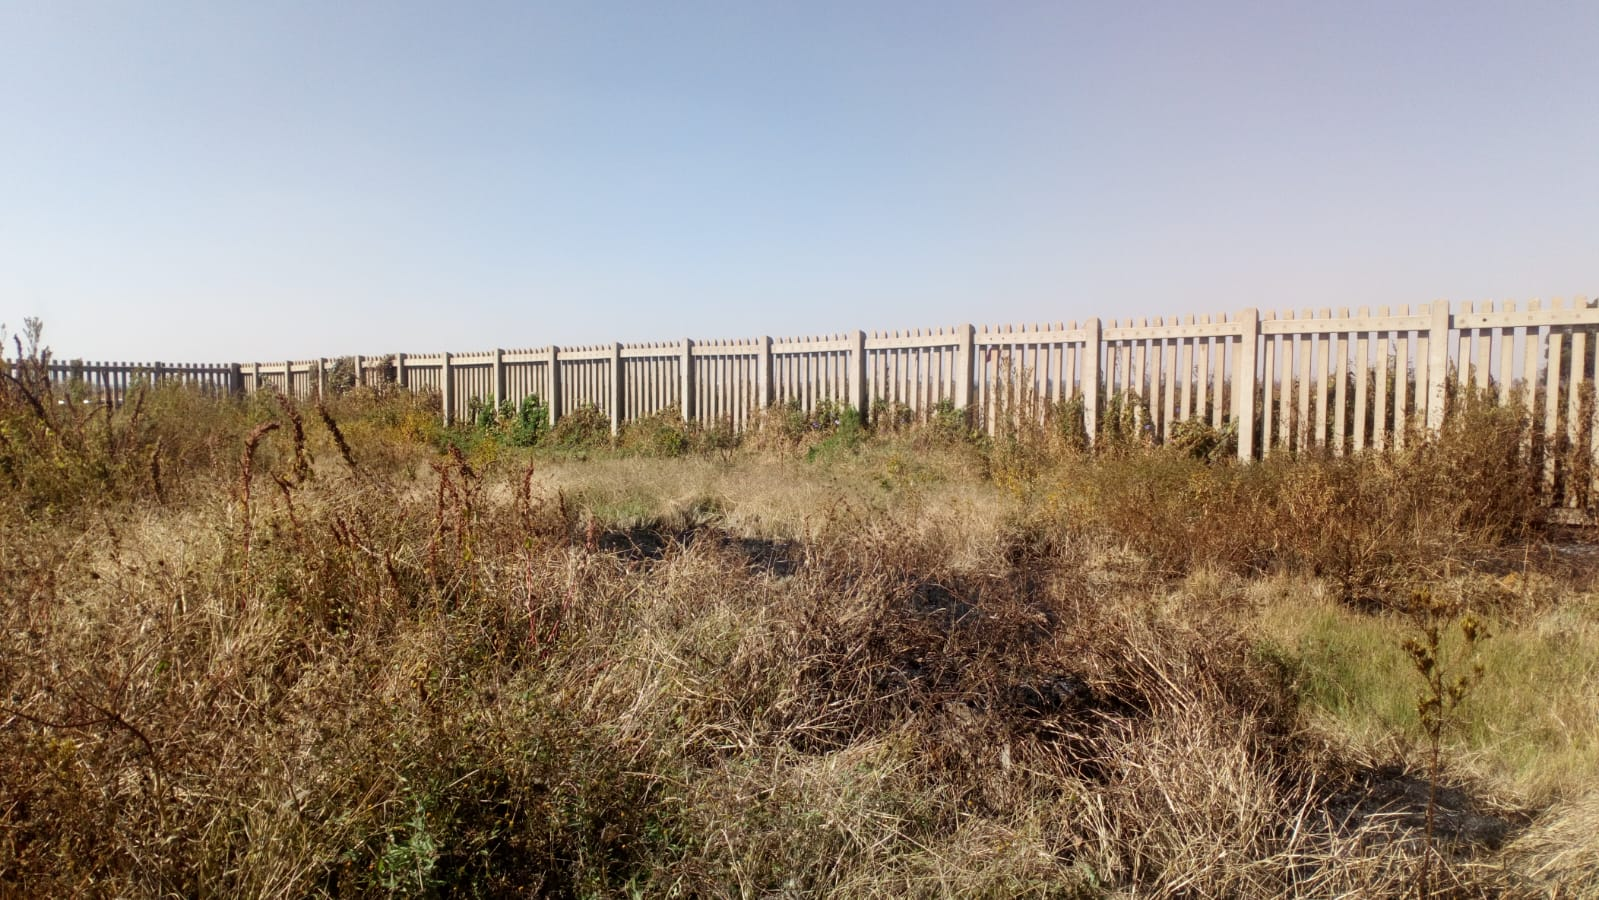
\includegraphics[width=\textwidth, height=3.4cm]{images/palisade-fencing-1.jpeg}
        \vspace{2pt}
        \centering
        {\scriptsize\bfseries\color{mhtextmuted} INFRASTRUCTURE SECURITY}\\
        {\footnotesize\bfseries\color{mhnavy} Palisade Perimeter Fencing}
    \end{tcolorbox}
\end{minipage}

\vspace{0.35cm}

\noindent
% Row 2 of Projects
\begin{minipage}[t]{0.315\textwidth}
    \begin{tcolorbox}[enhanced, colback=white, colframe=mhlightgray, boxrule=0.7pt, arc=3pt, left=0pt, right=0pt, top=0pt, bottom=6pt]
        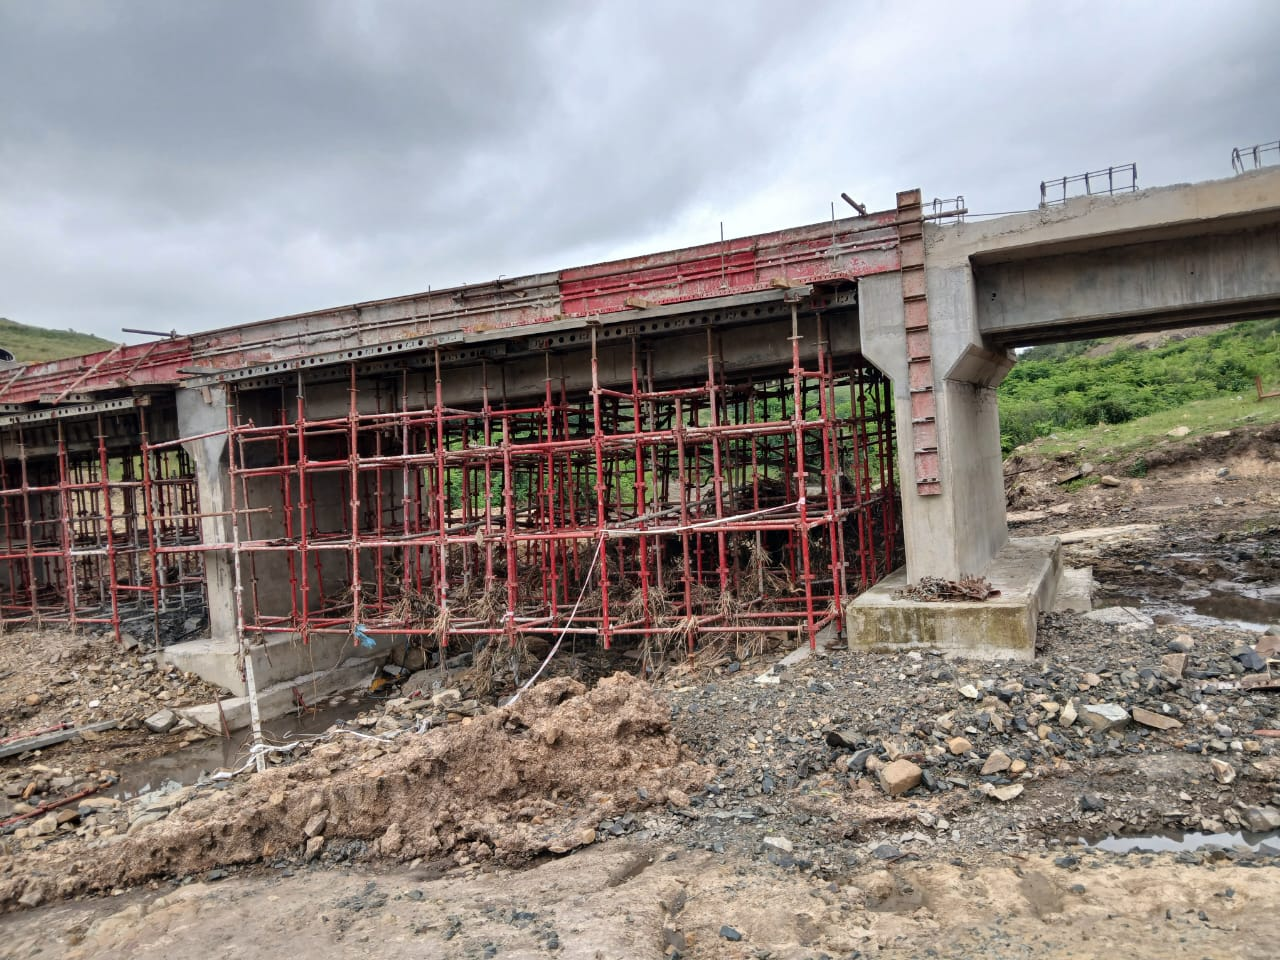
\includegraphics[width=\textwidth, height=3.4cm]{images/concrete-bridges-1.jpeg}
        \vspace{2pt}
        \centering
        {\scriptsize\bfseries\color{mhtextmuted} WATER \& BRIDGES}\\
        {\footnotesize\bfseries\color{mhnavy} Concrete Culvert Bridges}
    \end{tcolorbox}
\end{minipage}
\hfill
\begin{minipage}[t]{0.315\textwidth}
    \begin{tcolorbox}[enhanced, colback=white, colframe=mhlightgray, boxrule=0.7pt, arc=3pt, left=0pt, right=0pt, top=0pt, bottom=6pt]
        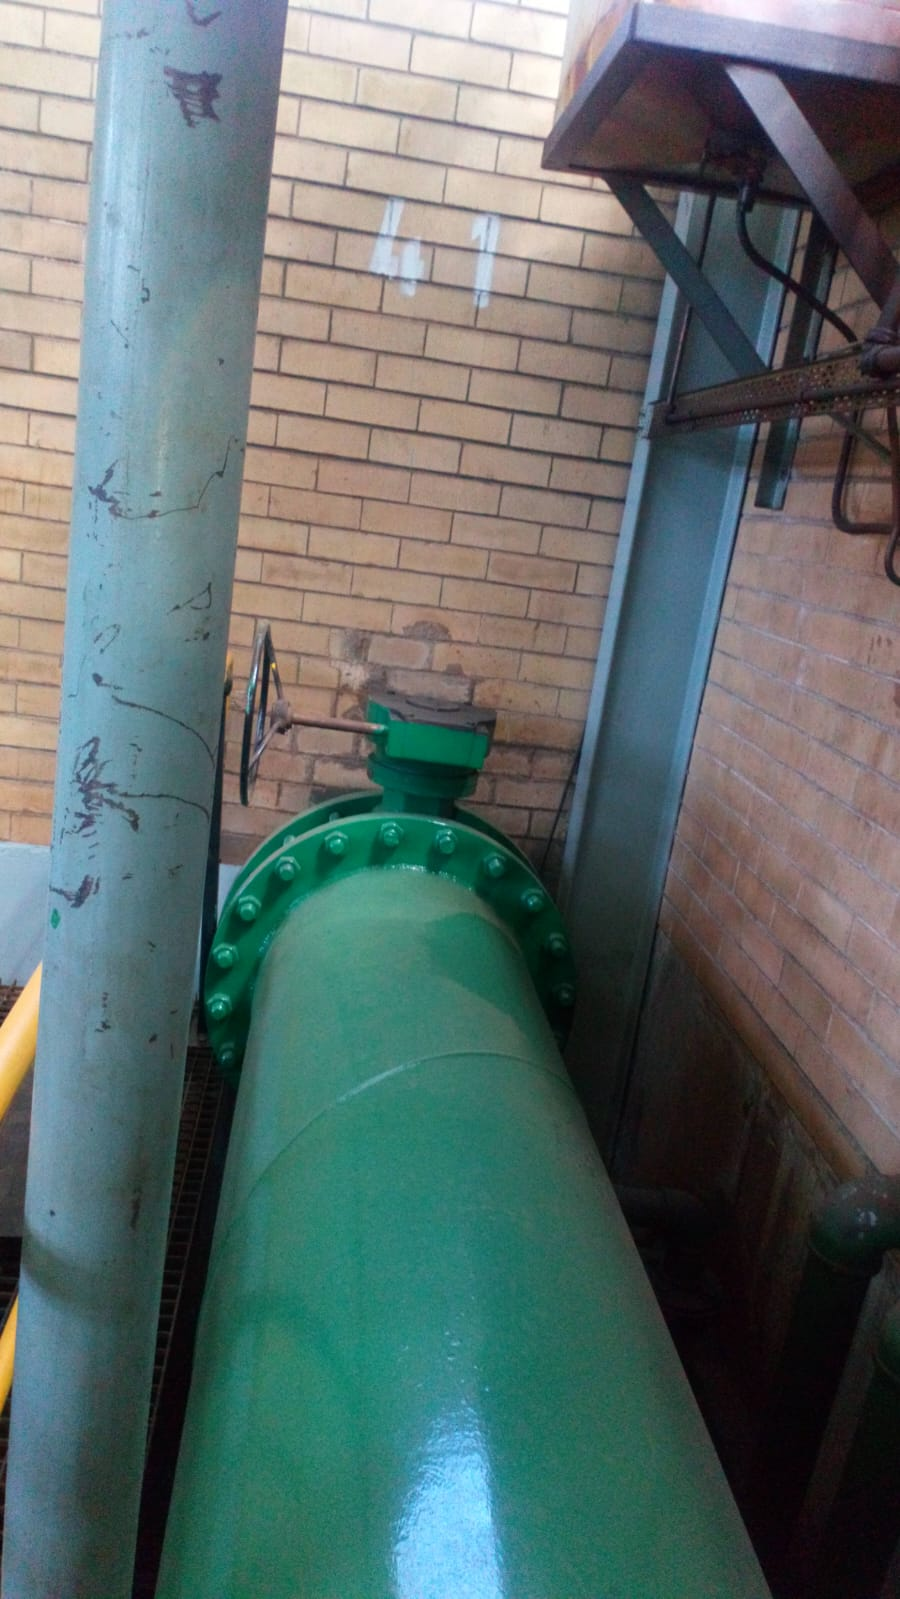
\includegraphics[width=\textwidth, height=3.4cm]{images/pumphouse-steel-pipe-works-1.jpeg}
        \vspace{2pt}
        \centering
        {\scriptsize\bfseries\color{mhtextmuted} MECHANICAL SERVICES}\\
        {\footnotesize\bfseries\color{mhnavy} Pumphouse Bulk Steel Piping}
    \end{tcolorbox}
\end{minipage}
\hfill
\begin{minipage}[t]{0.315\textwidth}
    \begin{tcolorbox}[enhanced, colback=white, colframe=mhlightgray, boxrule=0.7pt, arc=3pt, left=0pt, right=0pt, top=0pt, bottom=6pt]
        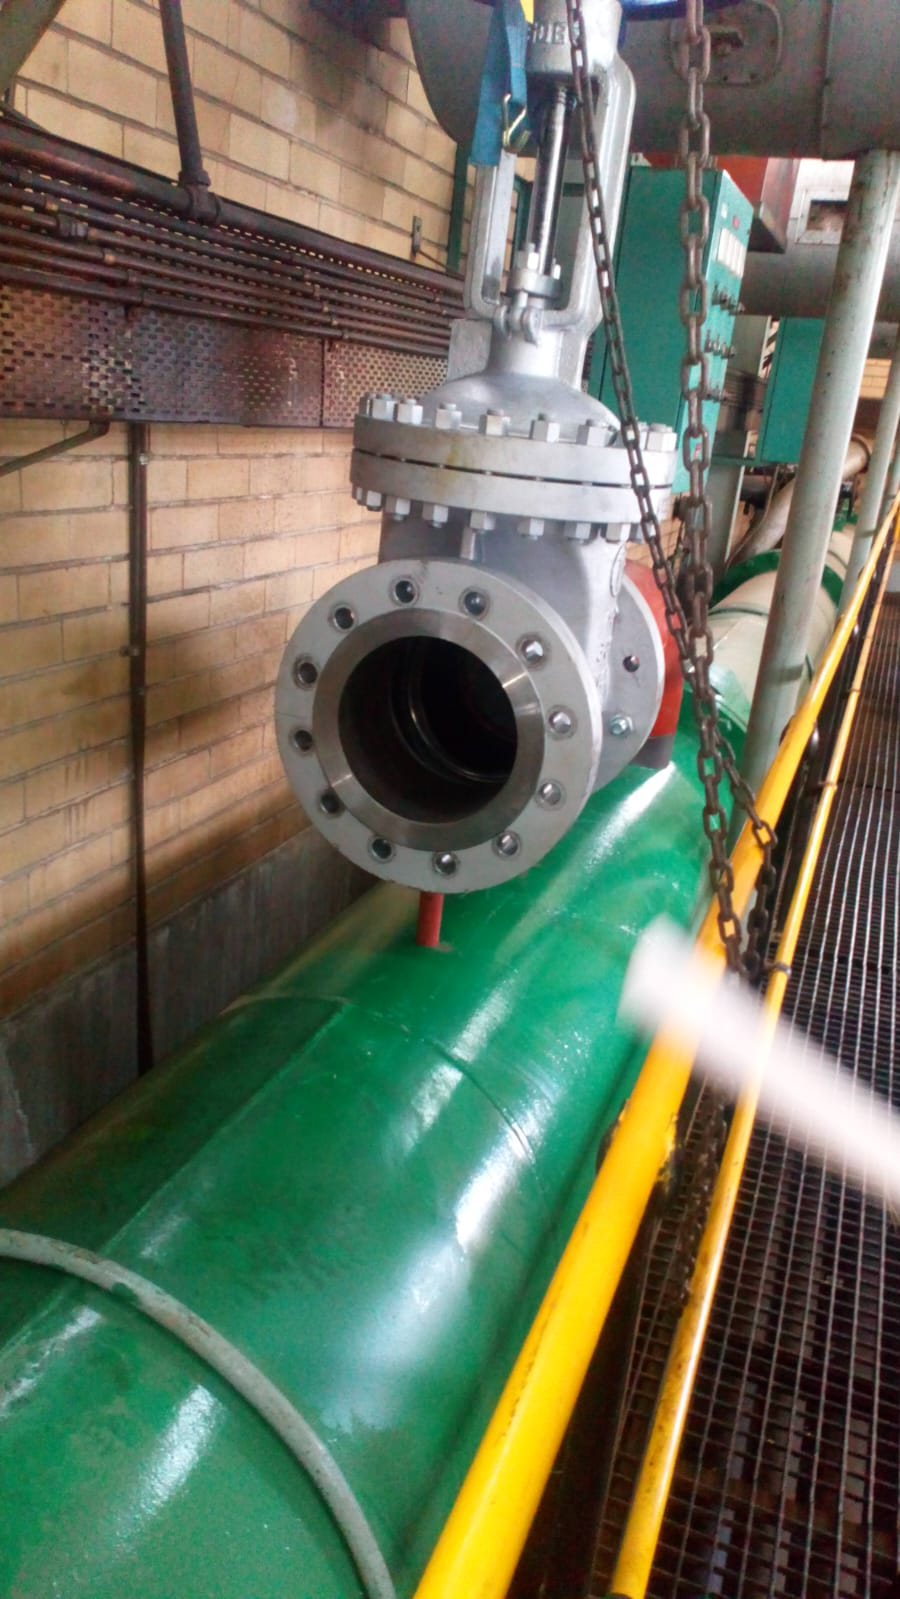
\includegraphics[width=\textwidth, height=3.4cm]{images/valves-and-groundwater-tanks-1.jpeg}
        \vspace{2pt}
        \centering
        {\scriptsize\bfseries\color{mhtextmuted} BULK WATER SYSTEMS}\\
        {\footnotesize\bfseries\color{mhnavy} Industrial Valve Chambers}
    \end{tcolorbox}
\end{minipage}

\vspace{0.35cm}

% Project Experience Summary Card
\begin{tcolorbox}[
    enhanced,
    colback=mhoffwhite,
    colframe=mhlightgray,
    boxrule=0.8pt,
    arc=4pt,
    left=10pt, right=10pt, top=8pt, bottom=8pt
]
    \fontsize{8.5pt}{11.5pt}\selectfont\color{mhtext}
    \textbf{Proven Track Record:} Makhaswa Holdings has successfully executed key civil infrastructure for provincial departments, metropolitan councils, and commercial clients --- including the \textbf{City of Tshwane}, housing agencies, and regional municipalities with flawless compliance and client satisfaction.
\end{tcolorbox}

\clearpage

% ===================================================
% PAGE 11 — CORPORATE SOCIAL INVESTMENT (CSI) & TRANSFORMATION
% ===================================================

\sectionbanner{Transformation}{Corporate Social Investment \& Community Empowerment}

\noindent
\begin{minipage}[t]{0.485\textwidth}
    \begin{brandcard}{Level 1 B-BBEE Transformation}
        As a 100\% black-owned enterprise with \textbf{135\% B-BBEE procurement recognition}, Makhaswa Holdings is a catalyst for economic transformation:

        \begin{itemize}[leftmargin=12pt, itemsep=3.5pt, label=\color{mhblue}$\blacktriangleright$]
            \item \textbf{Local Labour Sourcing:} Compulsory minimum of 30\% local community labour recruited on all site projects.
            \item \textbf{SMME Incubation:} Subcontracting civil packages to local emerging contractors with technical mentoring.
            \item \textbf{Youth \& Women Empowerment:} Targeted apprentice programs for female and youth civil technicians.
        \end{itemize}
    \end{brandcard}
\end{minipage}
\hfill
\begin{minipage}[t]{0.485\textwidth}
    \begin{brandcard}{Community Impact Initiatives (CSI)}
        We believe corporate success must uplift surrounding communities:

        \begin{itemize}[leftmargin=12pt, itemsep=3.5pt, label=\color{mhblue}$\blacktriangleright$]
            \item \textbf{School Infrastructure Upgrades:} Assisting local schools with access road grading, paving, and sanitation.
            \item \textbf{Water Access Support:} Providing water bowser relief during municipal water interruptions in host communities.
            \item \textbf{Accredited Skills Transfer:} Practical construction training, health and safety awareness, and equipment operation certifications.
        \end{itemize}
    \end{brandcard}
\end{minipage}

\vspace{0.4cm}

% Full-Width Commitment Banner
\begin{tcolorbox}[
    enhanced,
    colback=mhnavy,
    colframe=mhnavy,
    boxrule=0pt,
    arc=4pt,
    left=12pt, right=12pt, top=10pt, bottom=10pt,
    halign=center
]
    \color{white}
    {\large\bfseries\color{white} OUR PROMISE TO CLIENTS AND STAKEHOLDERS}\\[0.15cm]
    \fontsize{9pt}{13pt}\selectfont
    ``We do not simply complete contracts; we create lasting legacies. Our engineering builds communities, fosters inclusive economic participation, and delivers infrastructure that stands the test of time.''
\end{tcolorbox}

\vspace{0.35cm}

% Accreditation Row Badges
\noindent
\begin{minipage}{0.31\textwidth}
    \begin{tcolorbox}[enhanced, colback=mhoffwhite, colframe=mhlightgray, boxrule=0.7pt, arc=3pt, halign=center]
        
\includegraphics[height=1.1cm, keepaspectratio]{images/bbbee-logo.png}\\[2pt]
        {\tiny\bfseries\color{mhnavy} LEVEL 1 CONTRIBUTOR}
    \end{tcolorbox}
\end{minipage}
\hfill
\begin{minipage}{0.31\textwidth}
    \begin{tcolorbox}[enhanced, colback=mhoffwhite, colframe=mhlightgray, boxrule=0.7pt, arc=3pt, halign=center]
        
\includegraphics[height=1.1cm, keepaspectratio]{images/cidb-logo.png}\\[2pt]
        {\tiny\bfseries\color{mhnavy} GRADE 8 CE PE / 8 ME PE}
    \end{tcolorbox}
\end{minipage}
\hfill
\begin{minipage}{0.31\textwidth}
    \begin{tcolorbox}[enhanced, colback=mhoffwhite, colframe=mhlightgray, boxrule=0.7pt, arc=3pt, halign=center]
        
\includegraphics[height=1.1cm, keepaspectratio]{images/iso-logo.png}\\[2pt]
        {\tiny\bfseries\color{mhnavy} ISO 9001 / 14001 / 45001}
    \end{tcolorbox}
\end{minipage}

\clearpage

% ===================================================
% PAGE 12 — CONTACT DIRECTORY & MULTI-REGIONAL HUBS (BACK COVER)
% ===================================================

\thispagestyle{empty}

\begin{tikzpicture}[remember picture, overlay]
    % Clean, Solid Signature Navy Background (No Murky Gradients / No Rainbow Flags)
    \fill[mhnavy] (current page.north west) rectangle (current page.south east);
    
    % Subtle Clean Blue Bottom Keyline
    \fill[mhblue] (current page.south west) rectangle ([yshift=3mm]current page.south east);
\end{tikzpicture}

\pagecolor{mhnavy}
\color{white}

\begin{center}
    \vspace*{0.6cm}
    
    % Solid Logo Mounted in Crisp White Frame
    \begin{tcolorbox}[
        enhanced,
        colback=white,
        colframe=white,
        boxrule=0pt,
        arc=4pt,
        left=8pt, right=8pt, top=6pt, bottom=6pt,
        width=5.6cm,
        halign=center,
        drop shadow=black!30
    ]
        
\includegraphics[width=5.0cm, keepaspectratio]{images/logo.jpeg}
    \end{tcolorbox}

    \vspace{0.45cm}

    {\fontsize{24pt}{28pt}\selectfont\bfseries\color{white} CONTACT OUR OFFICES}
    \\[0.12cm]
    {\small\bfseries\color{mhbluelight} REACH OUT FOR TENDERS, JOINT VENTURES \& STRATEGIC PARTNERSHIPS}
\end{center}

\vspace{0.5cm}

% 4 Regional Hubs in 2x2 Grid (Clean Corporate Navy Cards)
\noindent
\begin{minipage}[t]{0.485\textwidth}
    \begin{tcolorbox}[
        enhanced, colback=mhnavy2, colframe=mhblue!40, boxrule=0.8pt, arc=4pt,
        left=9pt, right=9pt, top=9pt, bottom=9pt
    ]
        {\bfseries\color{white}\small PRETORIA HEAD OFFICE (GAUTENG)}\\[0.15cm]
        \fontsize{8pt}{11.5pt}\selectfont\color{white!90}
        869 Patryshond Street, Garsfontein, Pretoria, 0042\\
        \textbf{Telephone:} 012 944 1702\\
        \textbf{Direct Email:} info@makhaswaholdings.co.za
    \end{tcolorbox}
\end{minipage}
\hfill
\begin{minipage}[t]{0.485\textwidth}
    \begin{tcolorbox}[
        enhanced, colback=mhnavy2, colframe=mhblue!40, boxrule=0.8pt, arc=4pt,
        left=9pt, right=9pt, top=9pt, bottom=9pt
    ]
        {\bfseries\color{white}\small MIDRAND / JHB OFFICE (GAUTENG)}\\[0.15cm]
        \fontsize{8pt}{11.5pt}\selectfont\color{white!90}
        Riversands Incubation Hub, Riverside View Ext 15, Midrand\\
        \textbf{Telephone:} 011 568 0938\\
        \textbf{Direct Email:} info@makhaswaholdings.co.za
    \end{tcolorbox}
\end{minipage}

\vspace{0.3cm}

\noindent
\begin{minipage}[t]{0.485\textwidth}
    \begin{tcolorbox}[
        enhanced, colback=mhnavy2, colframe=mhblue!40, boxrule=0.8pt, arc=4pt,
        left=9pt, right=9pt, top=9pt, bottom=9pt
    ]
        {\bfseries\color{white}\small LIMPOPO REGIONAL OFFICE}\\[0.15cm]
        \fontsize{8pt}{11.5pt}\selectfont\color{white!90}
        197 Dudu Madisha Drive, Chroompark, Mokopane, 0656\\
        \textbf{Regional Inquiries:} info@makhaswaholdings.co.za
    \end{tcolorbox}
\end{minipage}
\hfill
\begin{minipage}[t]{0.485\textwidth}
    \begin{tcolorbox}[
        enhanced, colback=mhnavy2, colframe=mhblue!40, boxrule=0.8pt, arc=4pt,
        left=9pt, right=9pt, top=9pt, bottom=9pt
    ]
        {\bfseries\color{white}\small KWAZULU-NATAL REGIONAL OFFICE}\\[0.15cm]
        \fontsize{8pt}{11.5pt}\selectfont\color{white!90}
        71 Bertha Mkhize Street, Durban Central, Durban, 4001\\
        \textbf{Regional Inquiries:} info@makhaswaholdings.co.za
    \end{tcolorbox}
\end{minipage}

\vspace{0.4cm}

% Electronic Connect Banner
\begin{tcolorbox}[
    enhanced,
    colback=mhnavy2,
    colframe=mhblue,
    boxrule=1pt,
    arc=4pt,
    halign=center,
    left=10pt, right=10pt, top=10pt, bottom=10pt
]
    \color{white}
    \fontsize{8.5pt}{12.5pt}\selectfont
    \textbf{Direct Email:} info@makhaswaholdings.co.za
    \quad $\bullet$ \quad
    \textbf{WhatsApp Direct:} +27 81 359 8003
    \\[0.15cm]
    \textbf{Official Web Portal:} \href{https://www.makhaswaholdings.co.za}{\color{white}\underline{www.makhaswaholdings.co.za}}
\end{tcolorbox}

\vspace{0.8cm}

\begin{center}
    \fontsize{8pt}{11pt}\selectfont\color{white!80}
    \textbf{Makhaswa Holdings (Pty) Ltd} \ $\bullet$ \
    Registration: K2017/307900/07 \ $\bullet$ \
    VAT: 4840286027 \ $\bullet$ \
    CSD: MAAA0584716\\
    \textit{CIDB Grade 8 CE PE $\bullet$ 8 ME PE $\bullet$ 7 EB PE $\bullet$ 7 SB PE $\bullet$ 6 GB PE \ $\bullet$ \ Level 1 B-BBEE (135\%)}
\end{center}

\vspace{0.2cm}

\end{document}
